\documentclass[11pt]{article}

\usepackage[margin=0.95in]{geometry}
\usepackage{graphicx}
\usepackage[T1]{fontenc}
\usepackage[utf8]{inputenc}
\usepackage{lmodern}
\usepackage{microtype}
\usepackage{amsmath,amssymb,amsthm,mathtools}
\usepackage{booktabs}
\usepackage{longtable}
\usepackage{array}
\usepackage{multirow}
\usepackage{enumitem}
\usepackage{tikz}
\usetikzlibrary{arrows.meta,positioning,fit,calc,shapes.geometric,backgrounds}
\usepackage{hyperref}
\hypersetup{
  colorlinks=true,
  linkcolor=blue!55!black,
  citecolor=blue!55!black,
  urlcolor=blue!55!black
}
\usepackage[nameinlink,capitalise,noabbrev]{cleveref}

\setlength{\parskip}{0.55em}
\setlength{\parindent}{0pt}
\linespread{1.055}
\emergencystretch=2em

\newtheorem{definition}{Definition}
\newtheorem{proposition}{Proposition}
\newtheorem{assumption}{Assumption}
\newtheorem{claim}{Claim}
\newtheorem{designprinciple}{Design Principle}

\newcommand{\R}{\mathbb{R}}
\newcommand{\E}{\mathbb{E}}
\newcommand{\Prob}{\mathbb{P}}
\newcommand{\G}{\mathcal{G}}
\newcommand{\V}{\mathcal{V}}
\newcommand{\Ed}{\mathcal{E}}
\newcommand{\T}{\mathcal{T}}
\newcommand{\Z}{\mathcal{Z}}
\newcommand{\A}{\mathcal{A}}
\newcommand{\D}{\mathcal{D}}
\newcommand{\X}{\mathcal{X}}
\newcommand{\B}{\mathcal{B}}
\newcommand{\Kb}{k_{\mathrm B}}
\newcommand{\boltz}{\pi_\beta}
\newcommand{\uma}{U_{\mathrm{UMA}}}
\newcommand{\oracle}{\mathcal{O}}
\newcommand{\tokgt}{\mathrm{TokenGT}}
\newcommand{\got}{\mathrm{GoT}}
\newcommand{\gfn}{\mathrm{GFN}}
\newcommand{\mlip}{\mathrm{MLIP}}
\newcommand{\bioselfies}{\mathrm{BioSELFIES}}

\title{\textbf{Universal Graph Models, Oracle-Guided Flow Networks, and Structure-Training-Free Biomolecular Dynamics}\\
\large A research program for autoregressive graph-of-thought generation of temperature-conditioned physical trajectories without training on structure data}
\author{Amelie Schreiber}
\date{May 1, 2026}

\begin{document}
\maketitle

\begin{abstract}
This paper develops a rigorous research program around the following idea. Begin with the Tokenized Graph Transformer (TokenGT): a nearly standard Transformer that treats graph vertices and edges as tokens, uses graph-aware token embeddings and spectral positional encodings, and thereby lets ordinary attention reason over graphs. Train it first on sequence and graph corpora for biomolecules and small molecules, including FASTA-like protein, RNA, and DNA strings, SMILES, SELFIES, residue graphs, atom graphs, and genomic-context sequences, but do not train it on biomolecular structure data: no PDB/AFDB coordinate targets, no experimentally resolved conformational ensembles, no molecular dynamics trajectories, no structure-token targets, and no paired structure or trajectory targets. Then convert the model from token-space prediction to continuous embedding-space reasoning: the autoregressive decoder emits latent geometric hypotheses, soft contact maps, distance and torsion constraints, and graph-of-thought reasoning states. A GFlowNet-style objective, rather than standard reinforcement learning, trains the generator to sample terminal conformations or whole trajectories with probability proportional to a physically motivated reward. That reward is supplied by an oracle: primarily a universal machine-learned interatomic potential (MLIP), such as UMA, optionally wrapped with solvation, stereochemical, and thermodynamic corrections.

The core question is whether this can generate physical trajectories at specified temperatures while excluding structure data from policy training. The answer is nuanced. Without an oracle, the problem is not identifiable: sequence and chemical graph data alone do not determine a unique three-dimensional equilibrium distribution or kinetic process. With an energy-and-force oracle, however, one can formulate a principled active learning problem: learn a sampler over conformations and paths whose terminal or path distribution is proportional to a Boltzmann-, Onsager-Machlup-, or transition-path-style reward. TokenGT contributes a flexible representation for mixed biomolecular graphs; GFlowNets contribute distributional, mode-covering training; attention maps and edge-token attention contribute soft geometric hypotheses; and UMA-like MLIPs contribute scalable approximate physics. A central ablation collapses the input to a sequence-only linear graph: residues, bases, or atoms as ordered tokens, polymer-neighbor edges only, contact maps inferred from attention, and embedding-vector geometry refined by oracle scoring. This tests whether the model can learn structure-dynamics from sequence-only inputs once UMA-style feedback is available. A separate ablation studies geometry-as-token-features, in which available or oracle-generated distances, angles, torsions, local frames, or contact features are encoded as vertex and edge attributes. That ablation tests the value of geometric token features, but it is not the strict no-structure-input mainline. The resulting method is best understood not as learning structures or dynamics from examples, but as learning structure-dynamics by amortizing an oracle-defined statistical mechanics distribution.

The paper surveys and compares relevant methods: ESM3, gLM2, protein attention/contact-map work, Structure Language Models, BioEmu, Distributional Graphormer, DynaFold, latent diffusion on graph embeddings, AlphaFlow, P2DFlow, MDGen, Boltzmann Generators, small-molecule conformer generators, AlphaFold3, RoseTTAFold All-Atom, and nucleic-acid language models. It also develops a theoretical universal BioSELFIES tokenization layer for representing all biomolecular data through a robust SELFIES-style grammar, then refines that idea into a more efficient hybrid multiresolution tokenizer that keeps all-atom and side-chain dynamics where they matter. It then gives mathematical definitions, a proposed architecture, training objectives, temperature-conditioning mechanisms, implementation phases, evaluation protocols, failure modes, and a practical research plan for testing the hypothesis.
\end{abstract}

\tableofcontents
\newpage

\section{Executive Thesis}

The proposal in this paper is deliberately ambitious. It asks whether a Transformer that was originally designed to reason over graphs through clever tokenization can be made into a data-efficient, oracle-guided generator of biomolecular trajectories. The target setting is unusual: the model may train on sequence and graph corpora, and it may receive physical oracle feedback, but the mainline policy should not be trained on curated structure data of any kind: no PDB/AFDB coordinates, no structural token targets, no experimentally resolved conformational ensembles, no molecular dynamics (MD) trajectories, and no paired structure or trajectory targets. Its output should be a physical trajectory at a specified temperature, generated by autoregressive reasoning steps rather than by a diffusion sampler.

The strongest version of the thesis is:
\begin{quote}
\emph{A TokenGT-style autoregressive model, trained with a GFlowNet objective against an energy-and-force oracle, can learn to sample diverse biomolecular conformations and trajectory-like paths whose distribution approximates an oracle-defined finite-temperature ensemble, even when the policy is trained without structure data.}
\end{quote}

The precise claim is not that sequence tokens contain enough information to determine physics with no feedback. The stronger and more interesting claim is that a sequence-only \emph{input} may be enough once the learning loop includes a physical oracle. In that setting the model receives only a linear graph, uses attention maps and embedding-vector geometry to propose contacts and latent coordinates, queries UMA or a related oracle for energies and forces, and gradually learns the structure-dynamics distribution induced by the oracle. Sequence, graph, and chemical syntax pretraining provide priors over valid biomolecular objects. The oracle supplies the missing physics. GFlowNet training converts oracle evaluations into a distribution-matching signal. Autoregressive graph-of-thought decoding provides a computational scaffold for proposing, refining, branching, and selecting latent geometric hypotheses. Temperature enters both the target reward and the sampling entropy.

The first principle is therefore a boundary:
\begin{quote}
\emph{No structure data in policy training does not mean no physical information. It means the physical information enters through an oracle rather than through supervised structural examples.}
\end{quote}

This boundary matters because much of the modern literature achieves impressive conformational sampling by learning directly from static structures, MD simulations, or both. ESM3 learns discrete structure tokens from three-dimensional protein structures \cite{hayes2024esm3}. Structure Language Models encode protein conformations with a discrete VAE and model those codes with LMs \cite{lu2025slm}. BioEmu trains on AlphaFoldDB structures, more than 200 ms of MD simulation data, and experimental stability data \cite{lewis2025bioemu}. DynaFold and latent diffusion on graph embeddings train on trajectory or MD-derived structural data \cite{fan2025dynafold,sengar2025ldfpg}. AlphaFlow, P2DFlow, and MDGen learn flow or trajectory distributions from structure and dynamics data \cite{jing2024alphaflow,jin2025p2dflow,jing2024mdgen}. These methods are essential comparators, but they do not satisfy the strict no-structure-data version of the proposed constraint.

The research campaign has three main goals.

\begin{enumerate}[leftmargin=2em]
  \item Build the mathematical, biophysical, and deep learning foundation needed to state the approach without hand-waving.
  \item Compare existing generative dynamics and biomolecular foundation models by asking which ingredients can be borrowed without violating the no-structure-data training constraint, and which belong only in geometry-feature ablations.
  \item Quantify what additional non-structural graph information adds beyond a sequence-only linear graph under the same oracle budget.
  \item Give a pragmatic implementation plan and benchmark program that could falsify, repair, or support the proposed architecture.
\end{enumerate}

The main conclusion is a design recommendation. The most rigorous version is not to make attention maps literally ``be'' contact maps, nor to ask a Transformer to hallucinate Cartesian coordinates directly. Instead, the model should emit a \emph{latent physical path object}: soft contacts, distance intervals, torsions, local frames, uncertainty estimates, and low-dimensional conformation embeddings. A differentiable or semi-differentiable geometry solver maps these latent objects into coordinates. UMA or another MLIP scores the resulting coordinates. The GFlowNet learns to sample the latent path object in proportion to the oracle reward. This keeps the Transformer in the domain where it is strong, while pushing hard geometric and energetic constraints into modules designed for them.

\section{Research Lanes and Source Map}

The literature relevant to this project naturally separates into eight lanes. Each lane answers a different part of the question.

\begin{enumerate}[leftmargin=2em]
  \item \textbf{Graph Transformers and TokenGT.} TokenGT shows that a nearly pure Transformer can operate on arbitrary graphs if nodes and edges are converted into tokens and equipped with suitable type, identifier, and spectral embeddings \cite{kim2022tokengt}. This is the architectural seed.
  \item \textbf{Protein language models and contact emergence.} Work on protein LMs shows that attention and learned representations can encode contacts, secondary structure, mutational effects, and functional regions despite sequence-only pretraining \cite{rives2021biological,rao2021unsupervised,vig2021bertology,rao2021msa}. gLM2 extends this theme to mixed genomic context and reports unsupervised protein-protein interface signals via categorical Jacobians \cite{cornman2024omg}.
  \item \textbf{Structure-token and multimodal biomolecular LMs.} ESM3 and Structure Language Models demonstrate that discrete structure tokens make structural generation compatible with language modeling, but they require structure-derived tokenizers or structure training data, so they are comparators and sources of design ideas rather than training templates for the strict setting \cite{hayes2024esm3,lu2025slm}.
  \item \textbf{Equilibrium ensemble generators.} BioEmu, Distributional Graphormer, AlphaFlow, P2DFlow, and related diffusion/flow methods target conformational ensembles, often by learning from static structures, MD, and experimental thermodynamics; they are benchmark families, not permitted sources of training targets for the strict mainline \cite{lewis2025bioemu,zheng2024dig,jing2024alphaflow,jin2025p2dflow}.
  \item \textbf{Trajectory generators.} MDGen and DynaFold model trajectories or transition paths directly, but use trajectory data \cite{jing2024mdgen,fan2025dynafold}.
  \item \textbf{Energy-based and oracle-guided samplers.} Boltzmann Generators, GFlowNets, active learning with MLIPs, and path-sampling methods provide a framework for learning from energies, forces, rewards, and partition functions rather than demonstration trajectories \cite{noe2019boltzmann,bengio2021gflownet,bengio2023gflownet,malkin2022trajectory}.
  \item \textbf{Universal atomic oracles.} UMA-like MLIPs promise fast approximate energy and force evaluation across molecules, materials, and catalysts, but their domain, solvent treatment, long-range electrostatics, protonation, and biomolecular transfer limits must be handled explicitly \cite{wood2025uma}.
  \item \textbf{General biomolecular structure models.} AlphaFold3, RoseTTAFold All-Atom, Chai-1, Boltz-1, RhoFold+, RNA-FM, and Nucleotide Transformer show how representation learning has expanded from proteins to general biomolecular systems, although data for nucleic-acid dynamics remains sparse \cite{abramson2024af3,krishna2024rfaa,chaiteam2024chai1,wohlwend2024boltz1,shen2024rhofold,dallatorre2024nt}.
\end{enumerate}

\section{Definitions and Notation}

\subsection{Graphs, molecules, and sequence graphs}

\begin{definition}[Molecular graph]
A molecular graph is a tuple
\[
G=(V,E,\tau_V,\tau_E,x_V,x_E),
\]
where $V$ is a set of vertices, $E\subseteq V\times V$ is a set of edges, $\tau_V$ assigns vertex types, $\tau_E$ assigns edge types, and $x_V,x_E$ are optional vertex and edge features. For atom-level graphs, vertices are atoms and edges are bonds. For residue-level protein graphs, vertices are residues and edges include polymer adjacency, disulfides, known covalent modifications, and optional latent non-covalent candidate edges. For nucleic acids, vertices may be atoms, nucleotides, bases, sugars, or phosphate groups, depending on resolution.
\end{definition}

\begin{definition}[Linear graph]
A linear sequence of length $n$ is the path graph $P_n$ with vertices $\{1,\dots,n\}$ and edges $(i,i+1)$. FASTA, SMILES, and SELFIES strings can all be interpreted as sequences; SMILES and SELFIES can additionally be parsed into molecular graphs.
\end{definition}

\begin{definition}[Conformation]
For a molecular graph with $N$ atoms, a conformation is a coordinate matrix
\[
X=(r_1,\dots,r_N)^\top\in\R^{N\times 3}
\]
modulo global Euclidean motion. A conformation is physically valid only relative to chemistry: bond lengths, bond angles, stereochemistry, protonation state, charge state, excluded volume, and environment must be specified or marginalized.
\end{definition}

\begin{definition}[Trajectory]
A discrete trajectory at time step $\Delta t$ is a sequence
\[
\Gamma = (X_0,X_1,\dots,X_K)
\]
of conformations. A physical trajectory also includes momenta or velocities in full Hamiltonian dynamics, or a stochastic transition law in overdamped Langevin dynamics. A sequence of plausible conformations is not automatically a kinetic trajectory.
\end{definition}

\subsection{TokenGT tokenization}

TokenGT begins with a simple but powerful move: it treats graph nodes and edges as tokens and feeds the resulting token set to a standard Transformer. If $G=(V,E)$, then the token set is
\[
\T(G)=\{t_v:v\in V\}\cup\{t_e:e\in E\}.
\]
Each node token receives features derived from the node, and each edge token receives features derived from the edge and its endpoints. TokenGT uses type identifiers and orthonormal node identifiers built from graph positional encodings, typically involving Laplacian eigenvectors. A node token embedding has the schematic form
\[
h_v^{(0)} = W_V x_v + W_P p_v + W_T \tau_v,
\]
while an edge token for $e=(u,v)$ may use
\[
h_e^{(0)} = W_E x_e + W_{P,E}\,\phi(p_u,p_v) + W_T\tau_e,
\]
where $\phi$ may concatenate, add, multiply, or otherwise combine endpoint encodings.

The central reason this is attractive for biomolecules is that bonds, polymer adjacencies, contacts, hydrogen-bond hypotheses, base-pair hypotheses, disulfides, and long-range inferred relationships can all become first-class tokens. Attention is then not merely residue-to-residue attention; it includes node-node, node-edge, edge-node, and edge-edge interactions. This is important for contact-map reasoning because an entry of an attention matrix may involve an edge token that already represents a candidate physical relationship.

\begin{figure}[t]
\centering
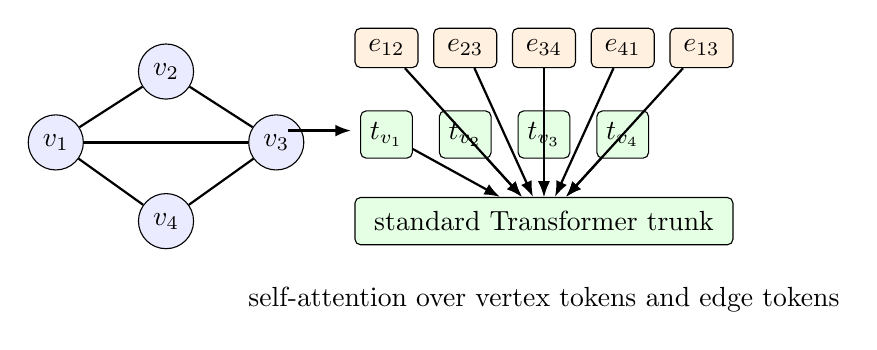
\begin{tikzpicture}[
  node/.style={circle,draw,minimum size=7mm,inner sep=0pt,fill=blue!8},
  edgeTok/.style={rectangle,draw,rounded corners=2pt,minimum width=8mm,minimum height=5mm,fill=orange!12},
  tok/.style={rectangle,draw,rounded corners=2pt,minimum height=6mm,fill=green!10},
  arrow/.style={-{Latex[length=2mm]},thick}
]
\node[node] (a) at (0,0) {$v_1$};
\node[node] (b) at (1.4,0.9) {$v_2$};
\node[node] (c) at (2.8,0) {$v_3$};
\node[node] (d) at (1.4,-1.0) {$v_4$};
\draw[thick] (a)--(b)--(c)--(d)--(a);
\draw[thick] (a)--(c);
\node[edgeTok] (e12) at (4.2,1.2) {$e_{12}$};
\node[edgeTok] (e23) at (5.2,1.2) {$e_{23}$};
\node[edgeTok] (e34) at (6.2,1.2) {$e_{34}$};
\node[edgeTok] (e41) at (7.2,1.2) {$e_{41}$};
\node[edgeTok] (e13) at (8.2,1.2) {$e_{13}$};
\node[tok] (t1) at (4.2,0.1) {$t_{v_1}$};
\node[tok] (t2) at (5.2,0.1) {$t_{v_2}$};
\node[tok] (t3) at (6.2,0.1) {$t_{v_3}$};
\node[tok] (t4) at (7.2,0.1) {$t_{v_4}$};
\node[tok,minimum width=4.8cm] (tr) at (6.2,-1.0) {standard Transformer trunk};
\draw[arrow] (2.95,0.15) -- (3.75,0.15);
\draw[arrow] (e12) -- (tr);
\draw[arrow] (e23) -- (tr);
\draw[arrow] (e34) -- (tr);
\draw[arrow] (e41) -- (tr);
\draw[arrow] (e13) -- (tr);
\draw[arrow] (t1) -- (tr);
\draw[arrow] (t2) -- (tr);
\draw[arrow] (t3) -- (tr);
\draw[arrow] (t4) -- (tr);
\node[align=center] at (6.2,-2.0) {self-attention over vertex tokens and edge tokens};
\end{tikzpicture}
\caption{TokenGT-style graph tokenization. Vertices and edges both become tokens. For biomolecules this means covalent bonds, polymer adjacencies, candidate contacts, H-bond hypotheses, base-pair hypotheses, and long-range graph relations can all participate directly in attention.}
\label{fig:tokengt}
\end{figure}

\subsection{Spectral positional encoding}

Let $A$ be the adjacency matrix of $G$, $D$ the degree matrix, and $L=D-A$ the unnormalized graph Laplacian. Other variants use the normalized Laplacian $I-D^{-1/2}AD^{-1/2}$. Spectral positional encodings use eigenvectors
\[
L u_k = \lambda_k u_k,
\]
with $p_v=(u_1(v),\dots,u_m(v))$ for vertex $v$. For a path graph, these eigenvectors are discrete sinusoidal modes, so spectral encodings generalize positional encodings from sequences to arbitrary graphs. The important caveats are sign ambiguity, eigenspace rotations for repeated eigenvalues, and sensitivity to graph perturbations. Practical implementations handle these by random sign augmentation, invariant combinations, learned projections, or multiple structural encodings.

For biomolecular graphs, spectral encodings are attractive but incomplete. They encode topology, not three-dimensional geometry. A linear protein chain and a folded protein share the same polymer path graph. Therefore, TokenGT's graph encoding can represent valid chemistry and sequence order, but it cannot by itself supply a fold. In the sequence-linear-graph setting, fold information must be learned from sequence priors, attention-derived contact hypotheses, embedding geometry, and oracle feedback. Enriched non-structural graphs can add chemistry, genomic context, covalent substructure, or typed biomolecular relations; their value should be measured against the linear-graph ablation. In a separate geometry-feature ablation, one may inject geometric token features such as distances, angles, torsions, local frames, or soft contact priors to measure how much explicit geometry changes the learning problem.

\section{Biophysical Foundations}

\subsection{Canonical ensembles}

For a molecular system at temperature $T$, define $\beta=(\Kb T)^{-1}$. If $U(X)$ is the potential energy of conformation $X$, the canonical equilibrium distribution is
\[
\pi_\beta(X)=\frac{1}{Z_\beta}\exp[-\beta U(X)],\qquad
Z_\beta=\int \exp[-\beta U(X)]\,dX.
\]
If momenta $P$ are included, the Hamiltonian is $H(X,P)=U(X)+K(P)$ and
\[
\pi_\beta(X,P)\propto \exp[-\beta H(X,P)].
\]
For conformational sampling, momenta are often integrated out, leaving the configurational distribution above.

The practical molecular biology version is more complex. A protein in water is not governed only by an intramolecular potential. The relevant marginal distribution is
\[
\pi_\beta(X_{\mathrm{solute}})\propto
\int \exp[-\beta U(X_{\mathrm{solute}},X_{\mathrm{solvent}},X_{\mathrm{ions}})]\,
dX_{\mathrm{solvent}}\,dX_{\mathrm{ions}},
\]
which defines an effective free energy surface
\[
F_\beta(X_{\mathrm{solute}})
=-\beta^{-1}\log \int \exp[-\beta U(X_{\mathrm{solute}},X_{\mathrm{env}})]\,dX_{\mathrm{env}}.
\]
Thus a vacuum MLIP energy is not generally a biomolecular free energy. This is one of the largest practical issues for UMA-guided biomolecular dynamics.

\subsection{Dynamics and path probabilities}

MD is not merely a sampler of endpoint conformations; it is a discretization of dynamics. In overdamped Langevin form,
\[
dX_t = -M\nabla U(X_t)\,dt + \sqrt{2\Kb T M}\,dW_t,
\]
where $M$ is a mobility matrix. A simple Euler discretization gives
\[
X_{k+1}=X_k - \Delta t\,M\nabla U(X_k)
 + \sqrt{2\Kb T\Delta t\,M}\,\xi_k,\qquad \xi_k\sim\mathcal{N}(0,I).
\]
This transition kernel has a path density. Up to discretization terms, a generated path $\Gamma=(X_0,\dots,X_K)$ can be scored by an Onsager-Machlup-like action
\[
S_\beta(\Gamma)
=
\sum_{k=0}^{K-1}
\frac{
\left\|X_{k+1}-X_k+\Delta t\,M\nabla U(X_k)\right\|^2_{M^{-1}}
}{
4\Kb T\Delta t
}
 + \text{correction terms}.
\]
This formula is central for the proposed method. If the model generates a whole trajectory, the oracle reward should not only ask whether each endpoint has low energy. It should also ask whether successive steps are dynamically plausible under a chosen stochastic dynamics.

\subsection{Temperature}

Temperature plays several roles:
\begin{enumerate}[leftmargin=2em]
  \item It defines the target equilibrium distribution through $\beta$.
  \item It sets the noise scale in Langevin dynamics.
  \item It influences conformational diversity and barrier crossing.
  \item It defines thermodynamic identities such as
  \[
  \operatorname{Var}_{\pi_\beta}[U]=\Kb T^2 C_V,
  \]
  where $C_V$ is heat capacity.
  \item It can be used as a conditioning variable for a generative model.
\end{enumerate}

The proposal has two temperatures that must not be conflated:
\[
T_{\mathrm{phys}}\quad\text{and}\quad T_{\mathrm{sample}}.
\]
$T_{\mathrm{phys}}$ is the physical temperature in the oracle-defined target distribution. $T_{\mathrm{sample}}$ is the model sampling temperature used in autoregressive decoding. One research objective is to calibrate them so that changing $T_{\mathrm{phys}}$ changes the reward and path action, while changing $T_{\mathrm{sample}}$ modulates exploration without destroying thermodynamic correctness. The final sampler may use a learned mapping
\[
\sigma_\theta(T_{\mathrm{phys}},s_k)
\]
for continuous action variance rather than a global softmax temperature.

\section{Deep Learning Foundations}

\subsection{Token-space reasoning versus embedding-space reasoning}

Classical language models generate discrete tokens. This is natural for text and usable for SMILES, SELFIES, amino-acid sequences, and structure-token models. The present proposal asks for continuous embedding vector reasoning. There are several possible meanings:

\begin{enumerate}[leftmargin=2em]
  \item The model is trained to predict continuous hidden states rather than discrete token IDs.
  \item The autoregressive actions are continuous vectors, such as latent conformation increments.
  \item The reasoning state is a graph of continuous hypotheses, not a string of symbolic thoughts.
  \item Discrete tokens still define the input graph and chemistry, but generated physical content is continuous.
\end{enumerate}

The most coherent interpretation is the fourth. Biomolecular syntax still needs discrete structure: atom types, residue identities, bases, bond types, chain breaks, stereochemistry tags, and graph topology. But conformational reasoning should be continuous because distances, torsions, local frames, energy gradients, and transition increments are continuous.

\subsection{Autoregressive continuous decoding}

Let $c$ denote the conditioning object: sequence, molecular graph, temperature, environment, and optional task prompt. Let $z_k$ be the latent geometric state at reasoning step $k$. An autoregressive continuous policy is
\[
p_\theta(z_{0:K}\mid c)=\prod_{k=0}^K p_\theta(z_k\mid z_{<k},c).
\]
For continuous actions, each factor can be a Gaussian, mixture density, normalizing-flow head, energy-based conditional, or diffusion-free stochastic head:
\[
p_\theta(z_k\mid z_{<k},c)
=\sum_{m=1}^{M}\alpha_{k,m}\,
\mathcal{N}(z_k;\mu_{k,m},\Sigma_{k,m}).
\]
This remains autoregressive even though outputs are not tokens.

The generated latent state should not be an opaque vector only. For physical scoring, it should decode into interpretable geometric objects:
\[
z_k \mapsto
\left(
D_k,\Theta_k,\Phi_k,C_k,Q_k,\Sigma_k
\right),
\]
where $D_k$ is a distance matrix or sparse distance set, $\Theta_k$ bond-angle constraints, $\Phi_k$ torsions, $C_k$ soft contacts, $Q_k$ local frames or coordinates, and $\Sigma_k$ uncertainty. A geometry solver then produces $X_k$.

\subsection{Graph-of-thought reasoning}

Graph-of-thought reasoning generalizes a chain of thoughts into a graph of intermediate hypotheses. In this setting a thought is not a sentence. It is a typed latent state such as:
\[
\begin{aligned}
\text{thought}\in
\{&\text{contact hypothesis},\text{torsion proposal},\text{local-frame update},\\
  &\text{energy critique},\text{branch merge}\}.
\end{aligned}
\]
The thought graph $H=(V_H,E_H)$ grows autoregressively. Each node is a latent proposal; each edge is a refinement, branching, merging, or evaluation relation. A terminal trajectory may be read from a path through $H$, while the whole graph records alternative hypotheses explored by the model.

This is a natural partner for GFlowNets. GFlowNets are trained on construction processes over compositional objects. A thought graph is exactly such a compositional object: the model incrementally constructs it, receives a reward at terminal states, and learns to sample high-reward objects in proportion to reward rather than collapsing to the single best object.

\section{GFlowNets for Physical Sampling}

\subsection{Core equations}

A GFlowNet is defined on a directed acyclic state graph with initial state $s_0$, terminal states $x\in\X$, forward policy $P_F(s'|s)$, backward policy $P_B(s|s')$, nonnegative flows $F(s)$, and terminal reward $R(x)>0$. The ideal flow equations are
\[
\sum_{s':s'\to s} F(s')P_F(s|s')
=
F(s)
=
\sum_{s'':s\to s''}F(s)P_F(s''|s),
\]
with terminal flow $F(x)=R(x)$. If the equations hold, terminal samples satisfy
\[
P_\theta(x)=\frac{R(x)}{Z},\qquad Z=\sum_{x\in\X}R(x).
\]
This is the key distinction from standard RL. RL typically maximizes expected reward and may collapse to the argmax. GFlowNets learn to sample diverse objects with probability proportional to reward.

The detailed balance objective enforces
\[
F(s)P_F(s'|s)=F(s')P_B(s|s')
\]
locally. The trajectory balance objective enforces, for a complete trajectory $\tau=(s_0\to s_1\to\dots\to x)$,
\[
\log Z_\theta+
\sum_{t=0}^{n-1}\log P_F(s_{t+1}|s_t)
-
\sum_{t=0}^{n-1}\log P_B(s_t|s_{t+1})
-
\log R(x)=0.
\]
The squared residual is minimized over sampled trajectories.

\subsection{Continuous actions}

For continuous latent actions $a_t\in\R^d$, probabilities become densities:
\[
P_F(s_{t+1}|s_t)\quad\leadsto\quad
p_F(a_t|s_t),
\]
and trajectory balance uses log densities. If state transitions include a deterministic map $s_{t+1}=f(s_t,a_t)$, one must account for Jacobians when comparing densities under different parameterizations. In a practical implementation, one can define both forward and backward actions in the same latent coordinate system to avoid accidental volume distortions.

\subsection{Reward design for conformations}

For equilibrium conformation generation at temperature $T$, a basic reward is
\[
R_T(X\mid G)=
\exp[-\beta E_{\mathrm{eff}}(X;G,T)]
\cdot \mathbf{1}_{\mathrm{valid}}(X)
\cdot R_{\mathrm{div}}(X)
\cdot R_{\mathrm{unc}}(X),
\]
where $E_{\mathrm{eff}}$ is an effective energy or free energy estimate, $\mathbf{1}_{\mathrm{valid}}$ encodes hard chemical constraints, $R_{\mathrm{div}}$ may encourage mode coverage only if it preserves the target distribution after correction, and $R_{\mathrm{unc}}$ may penalize oracle extrapolation.

For a trajectory, the reward should be path-based:
\[
R_T(\Gamma\mid G)=
\exp[-S_T(\Gamma)]
\prod_{k=0}^K \mathbf{1}_{\mathrm{valid}}(X_k)
\cdot R_{\mathrm{end}}(X_K)
\cdot R_{\mathrm{obs}}(\Gamma),
\]
where $S_T$ may be a discretized Langevin action, $R_{\mathrm{end}}$ may impose folding or transition endpoint conditions, and $R_{\mathrm{obs}}$ may encode optional experimental or task constraints.

If the goal is equilibrium sampling, the terminal distribution matters. If the goal is physical dynamics, transition probabilities, time correlations, and detailed balance matter. These are different research targets and should not be mixed casually.

\begin{figure}[t]
\centering
\resizebox{\textwidth}{!}{%
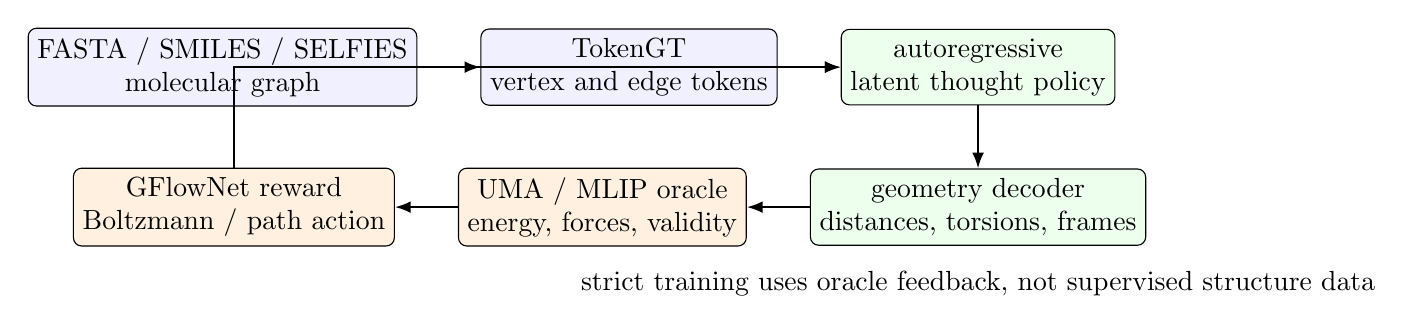
\begin{tikzpicture}[
  box/.style={draw,rounded corners=3pt,minimum height=8mm,align=center,fill=blue!6},
  gbox/.style={draw,rounded corners=3pt,minimum height=8mm,align=center,fill=green!7},
  obox/.style={draw,rounded corners=3pt,minimum height=8mm,align=center,fill=orange!12},
  arrow/.style={-{Latex[length=2mm]},thick}
]
\node[box,minimum width=2.8cm] (input) {FASTA / SMILES / SELFIES\\molecular graph};
\node[box,minimum width=2.8cm,right=0.8cm of input] (tok) {TokenGT\\vertex and edge tokens};
\node[gbox,minimum width=3.1cm,right=0.8cm of tok] (policy) {autoregressive\\latent thought policy};
\node[gbox,minimum width=3.1cm,below=0.8cm of policy] (geom) {geometry decoder\\distances, torsions, frames};
\node[obox,minimum width=3.0cm,left=0.8cm of geom] (oracle) {UMA / MLIP oracle\\energy, forces, validity};
\node[obox,minimum width=3.0cm,left=0.8cm of oracle] (reward) {GFlowNet reward\\Boltzmann / path action};
\draw[arrow] (input)--(tok);
\draw[arrow] (tok)--(policy);
\draw[arrow] (policy)--(geom);
\draw[arrow] (geom)--(oracle);
\draw[arrow] (oracle)--(reward);
\draw[arrow] (reward.north) |- (policy.west);
\node[align=center,below=0.2cm of geom] {strict training uses oracle feedback, not supervised structure data};
\end{tikzpicture}
}
\caption{Oracle-guided TokenGT-GFlowNet loop. Sequence and graph corpora supply syntax and priors. The generator proposes latent geometries and paths. A geometry decoder yields coordinates for scoring. The oracle supplies energy, force, validity, and uncertainty signals. GFlowNet training converts those rewards into distributional sampling.}
\label{fig:oracleloop}
\end{figure}

\section{The Identifiability Barrier}

The no-structure-data constraint is scientifically interesting precisely because it exposes an identifiability barrier.

\begin{proposition}[Non-identifiability without physical feedback]
Let $\D_{\mathrm{seq}}$ be a dataset containing only biomolecular sequences and molecular graphs, with no coordinate labels, structure tokens, dynamics labels, energies, or physical oracle queries. There exist distinct potentials $U_1$ and $U_2$ that assign the same probability to all observed sequences and graphs but induce different equilibrium distributions $\pi_{\beta,1}(X)$ and $\pi_{\beta,2}(X)$. Therefore, no learner trained only on $\D_{\mathrm{seq}}$ can identify the true conformational ensemble in general.
\end{proposition}

\begin{proof}
The observed data contain no coordinates. For any graph $G$, choose two potentials over conformations compatible with $G$, for example one favoring compact conformations and one favoring extended conformations. Both induce the same marginal distribution over $G$ if the graph distribution is fixed independently of coordinates. They therefore agree on all observations but disagree on $\pi_\beta(X|G)$. Any learner using only $\D_{\mathrm{seq}}$ receives identical evidence under both worlds.
\end{proof}

The practical consequence is simple: the proposed system cannot be defended as unaided sequence-only physics discovery. It can, however, be defended as \emph{sequence-only-input oracle-amortized statistical mechanics}. The oracle breaks non-identifiability by assigning energies, forces, constraints, or free energy estimates to generated conformations. The model then learns structure-dynamics from sequence-only or graph-augmented inputs by repeatedly proposing latent geometries, receiving physical feedback, and sampling from the oracle-defined distribution.

This also clarifies what counts as forbidden data. A database of PDB structures, AlphaFoldDB coordinates, conformer libraries, or MD trajectories used as training targets is forbidden in the strict setting. An MLIP trained elsewhere on quantum mechanical structures is an external physics oracle. Whether this is philosophically ``data-free'' depends on wording. The precise claim should be:
\begin{quote}
\emph{The TokenGT policy is trained without direct biomolecular structure examples, coordinate targets, structure-token targets, conformer datasets, or MD trajectories; it is trained from sequence/graph corpora and online oracle feedback.}
\end{quote}

\section{Tokenization Across Biomolecular Classes}

\subsection{Proteins}

Protein inputs can be represented at several resolutions.

\begin{longtable}{p{0.2\linewidth}p{0.34\linewidth}p{0.36\linewidth}}
\caption{Protein tokenization choices.}\\
\toprule
Resolution & Tokens & Strengths and risks\\
\midrule
\endfirsthead
\toprule
Resolution & Tokens & Strengths and risks\\
\midrule
\endhead
Amino-acid sequence & one residue token per amino acid, chain breaks, modifications & Scales well and matches FASTA corpora. Geometry is implicit. Side-chain and atom-level validity require decoding.\\
Residue graph & residue nodes, polymer edges, optional disulfide/crosslink/candidate contact edges & Natural for TokenGT. Can include edge tokens for known covalent or inferred non-covalent relations.\\
Backbone frame & residue tokens plus latent local frames, torsions, Ramachandran variables & Good compromise for folding dynamics. Requires geometry decoder and stereochemical constraints.\\
All atom & atom tokens and bond tokens, residue grouping metadata & Best for UMA scoring and chemistry. Long sequences become expensive; attention may need sparsification.\\
\bottomrule
\end{longtable}

Protein language models demonstrate that sequence-only training can induce structural signals. ESM-scale models learn features useful for structure and function \cite{rives2021biological}. Attention maps can predict contacts without supervised structure labels \cite{rao2021unsupervised}. BERTology-style analyses show attention heads connecting residues that are distant in sequence but close in space \cite{vig2021bertology}. The MSA Transformer shows the value of evolutionary families and tied row/column attention \cite{rao2021msa}. gLM2 extends the idea by using genomic context and reporting inter-protein interface signals from categorical Jacobians \cite{cornman2024omg}.

The proposed TokenGT model should borrow the following from protein LMs:
\begin{enumerate}[leftmargin=2em]
  \item masked and causal pretraining over residue strings;
  \item categorical Jacobian analyses to detect coevolution-like couplings;
  \item attention/contact calibration heads;
  \item genomic context when available;
  \item contrastive alignment between local sequence windows, residue graphs, and generated geometry.
\end{enumerate}

It should not assume that attention maps are calibrated physical contacts. They are hypotheses. They become physically meaningful only after calibration, geometry solving, and oracle feedback.

\subsection{Small molecules}

Small molecules have a different representational landscape. SMILES is compact and ubiquitous but syntactically fragile and non-unique \cite{weininger1988smiles}. SELFIES is robust: every SELFIES string decodes to a valid molecular graph, making it attractive for generative modeling \cite{krenn2020selfies}. Graph representations are often more physically direct because atoms and bonds are explicit.

For TokenGT, the small-molecule path is relatively clean:
\[
\text{SMILES/SELFIES}\to\text{RDKit molecular graph}\to
\text{atom tokens + bond tokens}\to\tokgt.
\]
Conformations can be generated through torsion angles rather than all Cartesian coordinates. For a fixed molecular graph, many degrees of freedom are constrained by chemistry. Let $\phi\in\R^m$ denote rotatable torsions. A conformation decoder can generate $\phi$ and then reconstruct coordinates with a distance-geometry or internal-coordinate engine. The oracle reward can use
\[
R_T(\phi|G)\propto\exp[-\beta U(X(\phi))].
\]
This is likely the best first proving ground for the approach because small molecules are shorter, have clearer constraints, and can be evaluated with multiple oracles: UMA, xTB, MMFF, ANI-like potentials, or quantum chemistry for small benchmarks.

\subsection{Nucleic acids}

Nucleic acids are the hardest and most scientifically valuable extension. RNA and DNA have strong sequence-structure relationships, but tertiary structure data are much scarcer than protein data, and dynamics are dominated by ions, solvent, hydrogen bonding, base stacking, base pairing, backbone torsions, and long-range electrostatics. RNA-FM and RhoFold+ show that RNA language models can support structure prediction under data scarcity \cite{shen2024rhofold}. Nucleotide Transformer and HyenaDNA show large-scale DNA representation learning, including long-context genomic modeling \cite{dallatorre2024nt,nguyen2023hyenadna}. Yet general nucleic-acid conformational dynamics models remain comparatively underdeveloped.

For nucleic acids, the TokenGT tokenizer should use hierarchical tokens:
\[
\begin{gathered}
\text{base tokens},\quad
\text{sugar tokens},\quad
\text{phosphate tokens},\\
\text{H-bond edge tokens},\quad
\text{base-pair edge tokens},\quad
\text{stacking edge tokens}.
\end{gathered}
\]
The model should also expose secondary-structure priors:
\[
C^{\mathrm{bp}}_{ij}\in[0,1],
\]
where $C^{\mathrm{bp}}_{ij}$ is a soft base-pair probability. These probabilities can come from classical RNA secondary structure algorithms, language model couplings, or learned heads, but they should remain hypotheses until oracle validation.

\subsection{General biomolecular complexes}

AlphaFold3 and RoseTTAFold All-Atom changed the field by treating complexes containing proteins, nucleic acids, small molecules, ions, and modifications as unified biomolecular structure prediction targets \cite{abramson2024af3,krishna2024rfaa}. This supports the long-term version of the present proposal: a single TokenGT framework should represent all biomolecular objects as typed graphs, with chain identity, covalent connectivity, polymer grammar, residue/base/atom hierarchy, and optional ligand graphs.

However, all-atom complex generation under finite-temperature dynamics is far harder than static structure prediction. The scaling burden comes from:
\begin{enumerate}[leftmargin=2em]
  \item large token counts if every atom and edge is explicit;
  \item solvent and ion degrees of freedom;
  \item long-range electrostatics;
  \item rare-event transitions;
  \item multiple protonation and tautomeric states;
  \item nontrivial kinetics and binding/unbinding pathways.
\end{enumerate}

Therefore, the implementation should begin with small molecules and peptides, then proteins, then RNA motifs, then mixed complexes.

\section{Theoretical Application: Universal BioSELFIES Tokenization}

A natural extension of the proposed program is to ask whether all biological input data can be tokenized through a SELFIES-like representation. SELFIES was designed for small molecules, where its central virtue is robustness: every SELFIES string decodes to a chemically valid molecular graph under the grammar \cite{krenn2020selfies}. For biomolecular dynamics, the attractive generalization is not merely to replace SMILES with SELFIES for ligands. It is to define a \emph{universal biomolecular SELFIES layer}, denoted here by $\bioselfies$, that serializes proteins, nucleic acids, glycans, cofactors, ions, ligands, post-translational modifications, and mixed complexes into a single constrained token language.

The important caveat is that literal small-molecule SELFIES is an atom-valence grammar, while biomolecular data are hierarchical. Proteins have residue, atom, chain, modification, and complex levels. Nucleic acids have base, sugar, phosphate, strand, base-pair, and stacking levels. Glycans have branching monosaccharide graphs and linkage stereochemistry. Therefore, a universal SELFIES approach should be understood as a \emph{SELFIES-style robust decoder} for typed biomolecular graphs:
\[
\delta_{\bioselfies}:\Sigma_{\bioselfies}^\star\to
\left(G_{\mathrm{bio}},m_{\mathrm{bio}}\right),
\]
where $\Sigma_{\bioselfies}$ is a finite or extensible alphabet of bracketed biomolecular tokens, $G_{\mathrm{bio}}$ is a typed covalent graph with hierarchy metadata, and $m_{\mathrm{bio}}$ stores chain identity, residue numbering, component type, protonation state, modification state, and environment annotations. The decoder should be total:
\[
\forall s\in \Sigma_{\bioselfies}^\star,\qquad
\delta_{\bioselfies}(s)\in \mathcal{G}_{\mathrm{valid}},
\]
possibly after deterministic repair, masking, or emission of an explicit null component. This totality is the core SELFIES principle: random or model-generated strings should not crash the chemistry parser or produce uninterpretable objects.

\subsection{Grammar design}

A practical $\bioselfies$ grammar can be organized as typed bracket tokens:
\[
\Sigma_{\bioselfies}
=
\Sigma_{\mathrm{atom}}
\cup\Sigma_{\mathrm{residue}}
\cup\Sigma_{\mathrm{base}}
\cup\Sigma_{\mathrm{link}}
\cup\Sigma_{\mathrm{branch}}
\cup\Sigma_{\mathrm{mod}}
\cup\Sigma_{\mathrm{component}}
\cup\Sigma_{\mathrm{env}}.
\]
Examples include:
\begin{center}
\begin{tabular}{lll}
\texttt{[AA:Ala]} & \texttt{[AA:Cys]} & \texttt{[RNA:G]}\\
\texttt{[DNA:T]} & \texttt{[MOD:phospho]} & \texttt{[LINK:peptide]}\\
\texttt{[LINK:phosphodiester]} & \texttt{[BRANCH:start]} & \texttt{[CHAIN:break]}
\end{tabular}
\end{center}
Small molecules can be represented by ordinary atom-level SELFIES tokens. Proteins and nucleic acids can be represented at residue/base level, atom level, or both. A hierarchical encoding might use residue tokens for long-range reasoning and expand selected residues to atom-level SELFIES subgraphs only when the geometry decoder needs all-atom detail.

The grammar should be implemented as a state machine. Let $q_t$ be the decoder state after reading tokens $s_{1:t}$. A token $a_t$ has preconditions and effects:
\[
q_{t+1}=F(q_t,a_t),\qquad
G_{t+1}=G_t+\Delta G(q_t,a_t),
\]
where $F$ enforces valence, polymer order, branch closure, chain boundaries, residue compatibility, and allowed modification sites. For example, a phosphorylation token may attach to Ser, Thr, Tyr, or other explicitly allowed modified residues; a phosphodiester link may connect nucleotide sugar-phosphate units; a peptide link may connect residue backbones; and a disulfide token may connect two cysteine side-chain handles if both are available. Invalid choices should map to a valid no-op, mask, repair token, or lower-priority attachment, preserving total decodability.

\subsection{Encoding biological hierarchy}

The decoder should return both a flat graph and a hierarchy:
\[
H_{\mathrm{bio}}
=
\left(
\text{atoms}\to\text{residues/bases/monomers}\to\text{chains}\to\text{complex}
\right).
\]
TokenGT can then receive multiple synchronized views:
\[
\bioselfies\ \text{tokens}
\quad\longrightarrow\quad
\text{vertex tokens}
\quad+\quad
\text{edge tokens}
\quad+\quad
\text{hierarchy tokens}.
\]
The vertex tokens may represent atoms, residues, bases, monosaccharides, ions, or coarse components. The edge tokens may represent covalent bonds, polymer adjacency, glycosidic linkages, candidate disulfides, component membership, or model-proposed non-covalent hypotheses. Crucially, no coordinates are introduced by this process. $\bioselfies$ supplies a robust symbolic object and a typed graph; geometry still emerges through attention, embedding-vector hypotheses, geometry decoding, and oracle feedback.

\subsection{SELFIES-only input for the oracle-guided model}

In the strictest $\bioselfies$ experiment, every datum is reduced to a robust string:
\[
s_{\bioselfies}
\to
\delta_{\bioselfies}(s_{\bioselfies})
=
(G_{\mathrm{cov}},m_{\mathrm{bio}})
\to
\tokgt.
\]
The model is not given FASTA, SMILES, PDB-derived graphs, MSA contacts, secondary-structure labels, or geometric features as separate channels. FASTA-like protein sequences, RNA/DNA strings, ligand SELFIES, glycans, and complexes are all first translated into $\bioselfies$. The downstream learning loop is unchanged:
\[
s_{\bioselfies}
\to
H_\theta
\to
\left(\hat{C},\hat{D},\hat{\Phi},\hat{Q}\right)
\to
X
\to
\oracle(X,T)
\to
R_T.
\]
Here $\hat{C}$ denotes attention-derived contacts, $\hat{D}$ distance hypotheses, $\hat{\Phi}$ torsions, and $\hat{Q}$ local frames or coordinate proposals. The GFlowNet objective trains the sampler to assign probability proportional to the oracle reward. In this sense, $\bioselfies$ becomes the universal symbolic substrate, while UMA-like scoring remains the physical teacher.

\subsection{Trajectory and thought serialization}

One can go further and use $\bioselfies$ not only for biological inputs but also for discrete graph-of-thought states. A thought trace can be serialized by special tokens:
\begin{center}
\begin{tabular}{lll}
\texttt{[THOUGHT:start]} & \texttt{[CONTACT:i:j]} & \texttt{[TORSION:k]}\\
\texttt{[TEMP:300K]} & \texttt{[STEP]} & \texttt{[THOUGHT:end]}
\end{tabular}
\end{center}
These should not be treated as supervised structure tokens. They are internal action tokens or logging tokens for the autoregressive policy. Continuous values, such as torsion angles or distance intervals, can be emitted through continuous heads attached to the discrete thought token:
\[
a_t=(\sigma_t,\xi_t),\qquad
\sigma_t\in\Sigma_{\mathrm{thought}},\quad
\xi_t\in\R^d.
\]
The discrete part $\sigma_t$ says what type of latent operation is being proposed; the continuous part $\xi_t$ gives the geometric value. This preserves the user's desired continuous embedding-vector reasoning while allowing every symbolic component of the system to live in a robust SELFIES-like token language.

\subsection{Advantages}

Universal $\bioselfies$ tokenization has several theoretical advantages:
\begin{enumerate}[leftmargin=2em]
  \item \textbf{Validity by construction.} Generated symbolic biomolecules decode to valid typed graphs rather than malformed strings.
  \item \textbf{One interface for many biomolecules.} Proteins, RNA, DNA, ligands, glycans, ions, and modifications can share a single tokenizer and parser contract.
  \item \textbf{Natural compatibility with TokenGT.} A decoded $\bioselfies$ object immediately yields vertex tokens, edge tokens, type embeddings, and hierarchy metadata.
  \item \textbf{Clean ablations.} One can compare FASTA/SMILES/native graph inputs against a $\bioselfies$-only pipeline under matched oracle budgets.
  \item \textbf{Generative repair.} Invalid biological edits can be mapped to valid repairs, enabling exploration without parser failure.
  \item \textbf{Compositional scaling.} Rare biomolecular complexes can be represented by composing known component grammars.
\end{enumerate}

\subsection{Risks and limits}

The main risk is false universality. A robust symbolic grammar does not make the physical problem easy. It only guarantees a valid decoded graph. It does not guarantee correct protonation, tautomeric state, solvation, metal coordination, membrane context, or conformational ensemble. For proteins and nucleic acids, residue-level $\bioselfies$ hides atom-level stereochemistry unless the decoder expands residues with chemically faithful templates. For complexes, non-covalent interactions are not fixed graph edges in the same way covalent bonds are; they should be proposed, scored, and revised rather than baked in from structure labels.

Thus the correct theoretical claim is:
\begin{quote}
\emph{Universal SELFIES-style tokenization can provide a robust, unified symbolic interface for biomolecular graph construction, but structure-dynamics still must be learned through oracle-guided latent geometry and temperature-conditioned sampling.}
\end{quote}

\subsection{Experimental comparison}

The $\bioselfies$ application should be evaluated as another representation ablation:
\[
\begin{aligned}
&\text{native input}
\quad\text{vs.}\quad
\text{linear sequence graph}\\
&\quad\text{vs.}\quad
\bioselfies\text{-only}
\quad\text{vs.}\quad
\bioselfies+\text{enriched graph}.
\end{aligned}
\]
Metrics should include parser validity, graph fidelity, oracle calls to valid geometry, basin coverage, temperature calibration, and independent-oracle agreement. If $\bioselfies$-only matches native graph inputs, the representation has achieved a powerful unification. If it lags, the gap identifies what biological information is lost in serialization and should guide grammar refinement.

\section{Efficient Hybrid Tokenization Beyond All-SELFIES}

The all-$\bioselfies$ construction is theoretically clean, but it is not necessarily the most efficient representation for oracle-guided dynamics. SELFIES is excellent for robust symbolic generation of atom-bond graphs, especially for ligands and small molecules. Biomolecular dynamics, however, often depends on multiscale structure: protein backbones move slowly, side chains reorient locally, ligands have dense atom-level chemistry, nucleic acids mix base-pairing with sugar-phosphate flexibility, and only a small subset of atoms usually participates in a given binding or transition event. Tokenizing every atom of every biomolecular component as SELFIES would waste context length and blur natural physical hierarchies.

The efficient alternative is a \emph{hybrid multiresolution tokenizer}. It keeps SELFIES in the system, but uses it where it is strongest: small molecules, cofactors, covalent modifications, glycans, and atom-level patches. Proteins and nucleic acids receive hierarchical tokens, with all-atom expansion only where local dynamics or ligand interactions require it.

\subsection{Token families}

Define a token set
\[
\mathcal{T}_{\mathrm{hyb}}
=
\mathcal{T}_{\mathrm{poly}}
\cup
\mathcal{T}_{\mathrm{atom}}
\cup
\mathcal{T}_{\mathrm{patch}}
\cup
\mathcal{T}_{\mathrm{lig}}
\cup
\mathcal{T}_{\mathrm{HB}}
\cup
\mathcal{T}_{\mathrm{int}}
\cup
\mathcal{T}_{\bioselfies}.
\]
Here $\mathcal{T}_{\mathrm{poly}}$ contains residue, base, sugar, phosphate, chain, and domain tokens; $\mathcal{T}_{\mathrm{atom}}$ contains explicit atom tokens; $\mathcal{T}_{\mathrm{patch}}$ marks local all-atom expansions; $\mathcal{T}_{\mathrm{lig}}$ contains ligand tokens; $\mathcal{T}_{\mathrm{HB}}$ contains hydrogen-bond donor, acceptor, virtual-hydrogen, and hydrogen-bond edge tokens; $\mathcal{T}_{\mathrm{int}}$ contains other candidate interaction-edge tokens; and $\mathcal{T}_{\bioselfies}$ contains SELFIES or BioSELFIES tokens for robust serialization.

The decoded object is not one flat sequence but a hierarchy:
\[
\mathcal{H}
=
\left(
G_{\mathrm{coarse}},
G_{\mathrm{atom}}^{\mathrm{patch}},
G_{\mathrm{lig}},
E_{\mathrm{HB}},
E_{\mathrm{int}},
\rho
\right),
\]
where $G_{\mathrm{coarse}}$ is the residue/base-level graph, $G_{\mathrm{atom}}^{\mathrm{patch}}$ contains explicit all-atom neighborhoods, $G_{\mathrm{lig}}$ is the ligand graph decoded from SELFIES or standard atom-bond tokens, $E_{\mathrm{HB}}$ contains candidate hydrogen-bond edges, $E_{\mathrm{int}}$ contains other candidate non-covalent edges, and $\rho$ records resolution metadata.

\subsection{Protein side-chain and ligand dynamics}

For proteins, the efficient base representation is residue-level:
\[
v_i=(\text{amino acid}_i,\text{chain}_i,\text{index}_i,\text{state}_i).
\]
Backbone dynamics are represented by internal-coordinate heads:
\[
(\phi_i,\psi_i,\omega_i)\sim p_\theta(\cdot\mid h_i,T),
\]
while side-chain dynamics are represented by rotamer or torsion heads:
\[
\chi_i=(\chi_{i1},\dots,\chi_{im_i})
\sim p_\theta(\cdot\mid h_i,H_{\mathrm{local}},T).
\]
Most residues do not need explicit atom tokens at every reasoning step. Instead, the model opens an all-atom patch when local physics requires it:
\[
\mathrm{open\_patch}(i,r)
\Rightarrow
G_{\mathrm{atom}}^{(i,r)}
=
\{a:\operatorname{dist}_{\mathrm{graph}}(a,i)\le r\}.
\]
The distance here is graph distance or model-proposed neighborhood distance, not a supervised structural distance. The patch may include the side-chain atoms of residue $i$, nearby covalent atoms, a ligand, a metal, or a candidate interaction partner.

Ligands remain a natural SELFIES use case:
\[
s_{\mathrm{lig}}^{\mathrm{SELFIES}}
\to
G_{\mathrm{lig}}
\to
\{\text{ligand atom tokens},\text{ligand bond tokens}\}.
\]
The protein-ligand interface is then represented by explicit interaction-edge tokens:
\[
e_{ia}^{\mathrm{int}}
=
\left(
\text{residue/atom } i,\,
\text{ligand atom } a,\,
\tau_{\mathrm{int}},\,
\alpha_{ia}
\right),
\]
where $\tau_{\mathrm{int}}$ may denote salt-bridge candidate, hydrophobic contact, $\pi$-stacking, metal coordination, steric clash, or covalent-warhead candidate, and $\alpha_{ia}$ is a confidence or logit generated by attention/Jacobian heads. These edge tokens are hypotheses. UMA or a hybrid oracle scores the reconstructed all-atom coordinates and determines whether the hypothesized interaction is physically useful.

Hydrogen bonds should be promoted from generic contacts to first-class typed edge tokens. For donor $D$, hydrogen $H$, and acceptor $A$, an H-bond hypothesis can be represented as
\[
e_{DHA}^{\mathrm{HB}}
=
\begin{aligned}[t]
(&D,H,A,\tau_D,\tau_A,q_D,q_A,\\
&r_{DA},r_{HA},\theta_{DHA},\alpha_{DHA}),
\end{aligned}
\]
where $\tau_D$ and $\tau_A$ encode donor and acceptor chemistry, $q_D$ and $q_A$ encode local charge/protonation features, $r_{DA}$ and $r_{HA}$ are reconstructed or oracle-returned distances, $\theta_{DHA}$ is the donor-hydrogen-acceptor angle, and $\alpha_{DHA}$ is the model confidence. If hydrogens are implicit in the input graph, the decoder instantiates virtual hydrogens from protonation-state templates before oracle scoring. Thus, sequence-only training still receives no structural target, but the generated trajectory is judged on whether its proposed donor/acceptor geometry can be physically realized.

A lightweight H-bond consistency term can be added to the oracle-shaped reward:
\[
\mathcal{V}_{\mathrm{HB}}(\Gamma)
=
\sum_{e\in E_{\mathrm{HB}}(\Gamma)}
\left[
\operatorname{ReLU}(r_{HA}(e)-r_{\max})^2
+
\operatorname{ReLU}(\theta_{\min}-\theta_{DHA}(e))^2
+
\mathbb{I}_{\mathrm{invalid}}(e)
\right],
\]
where $\mathbb{I}_{\mathrm{invalid}}$ flags chemically impossible donor/acceptor assignments. This term should be used as oracle feedback, not as supervised structure training.

\subsection{Dynamic patch refinement}

The tokenizer can be adaptive. At thought step $k$, the policy decides which regions need more resolution:
\[
a_k^{\mathrm{res}}
\in
\begin{aligned}[t]
\{&
\mathrm{keep\ coarse},\mathrm{open\ atom\ patch},
\mathrm{close\ patch},\\
&\mathrm{expand\ ligand},\mathrm{add\ HB\ edge},
\mathrm{add\ interaction\ edge}\}.
\end{aligned}
\]
This produces a variable-resolution state
\[
s_k=(G_{\mathrm{coarse}},G_{\mathrm{atom},k}^{\mathrm{patch}},G_{\mathrm{lig}},E_{\mathrm{HB},k},E_{\mathrm{int},k},Z_k,T).
\]
The reward should penalize unnecessary token expansion:
\[
\log R_T^{\mathrm{eff}}(\Gamma)
=
\log R_T^{\mathrm{phys}}(\Gamma)
-\lambda_{\mathrm{HB}}\mathcal{V}_{\mathrm{HB}}(\Gamma)
-\lambda_{\mathrm{tok}}\sum_k |\mathcal{T}_k|
-\lambda_{\mathrm{patch}}\sum_k |G_{\mathrm{atom},k}^{\mathrm{patch}}|.
\]
This makes efficiency part of the learning problem. The model is rewarded for opening all-atom detail only when it improves physical plausibility, mode coverage, or oracle score.

\subsection{Nucleic-acid hybrid tokenization}

Nucleic acids need a parallel but distinct hierarchy. The efficient base representation separates base, sugar, and phosphate:
\[
v_i^{\mathrm{NA}}
=
(\text{base}_i,\text{sugar}_i,\text{phosphate}_i,\text{strand}_i).
\]
The principal dynamic variables are:
\[
\eta_i=
(\alpha_i,\beta_i,\gamma_i,\delta_i,\epsilon_i,\zeta_i,\chi_i,p_i),
\]
where $\alpha,\dots,\zeta$ are backbone torsions, $\chi$ is the glycosidic torsion, and $p_i$ denotes sugar pucker. Candidate interaction edges include:
\[
\tau_{\mathrm{NA}}
\in
\begin{aligned}[t]
\{&
\text{Watson-Crick pair},\text{wobble pair},
\text{noncanonical pair},\\
&\text{base-pair H-bond},\text{sugar-phosphate H-bond},\\
&\text{base stacking},\text{ion bridge},
\text{protein contact},\text{ligand contact}\}.
\end{aligned}
\]
All-atom patches should be opened around base triples, bulges, ligand-binding pockets, ribozymes, ions, or protein-RNA interfaces. This is more efficient than atomizing the entire RNA or DNA molecule, while preserving the ability to model sugar pucker, base stacking, hydrogen bonding, and ion-sensitive dynamics when those details matter.

\subsection{Where SELFIES remains essential}

The hybrid tokenizer does not discard SELFIES. It assigns SELFIES a sharper role:
\begin{enumerate}[leftmargin=2em]
  \item \textbf{Ligands and cofactors.} Small molecules are decoded from SELFIES into atom-bond graphs.
  \item \textbf{Covalent modifications.} Post-translational modifications, nucleotide modifications, glycans, and covalent warheads can be represented as SELFIES subgraphs attached to residue/base handles.
  \item \textbf{Patch serialization.} Opened all-atom patches can be serialized as local BioSELFIES strings for replay, caching, and generative editing.
  \item \textbf{Fallback validity.} If a generated local chemical edit is ambiguous, the model can route it through the SELFIES/BioSELFIES decoder to guarantee a valid graph.
  \item \textbf{Ablation control.} The all-$\bioselfies$ tokenizer remains a clean baseline against which the hybrid representation can be compared.
\end{enumerate}

\subsection{Efficiency criterion}

Let $N_{\mathrm{atom}}$ be the number of all atoms and $N_{\mathrm{patch}}$ the number of atoms currently expanded in patches. A full atom-level tokenizer has cost roughly
\[
C_{\mathrm{all}}
\approx
O((N_{\mathrm{atom}}+|E_{\mathrm{atom}}|)^2)
\]
under dense attention. The hybrid tokenizer has cost
\[
C_{\mathrm{hyb}}
\approx
O((N_{\mathrm{coarse}}+|E_{\mathrm{coarse}}|+N_{\mathrm{patch}}+N_{\mathrm{lig}}+|E_{\mathrm{HB}}|+|E_{\mathrm{int}}|)^2),
\]
with $N_{\mathrm{patch}}\ll N_{\mathrm{atom}}$ for local binding, side-chain rearrangement, or nucleic-acid motif tasks. The scientific question is whether this lower token cost preserves all-atom accuracy near active interfaces.

\subsection{Experimental comparison}

The representation comparison should include:
\[
\begin{aligned}
&\bioselfies\text{-only}
\quad\text{vs.}\quad
\text{full all-atom graph}\\
&\quad\text{vs.}\quad
\text{hybrid multiresolution}
\quad\text{vs.}\quad
\text{hybrid plus geometry features}.
\end{aligned}
\]
Metrics should include oracle calls, wall-clock cost, peak token count, side-chain rotamer recovery, ligand pose stability, protein-ligand contact realism, H-bond geometry and occupancy, nucleic-acid base-pair and stacking consistency, temperature calibration, and independent-oracle agreement. The desired result is not that the hybrid tokenizer always beats all-atom tokenization. The desired result is a Pareto improvement: similar physical fidelity at much lower token and oracle budget for tasks whose important dynamics are localized.

\section{Ablation: Sequence-Only Linear Graphs}

The most severe no-structure-data setting should be made explicit. The input is not an enriched biomolecular graph, not an MSA contact graph, not a predicted secondary-structure graph, and not a database-derived structural graph. It is only the sequence represented as a linear graph:
\[
G_{\mathrm{lin}}=(V,E_{\mathrm{lin}}),\qquad
V=\{1,\dots,L\},\qquad
E_{\mathrm{lin}}=\{(i,i+1):1\le i<L\}.
\]
For proteins, $V$ contains amino-acid tokens. For RNA and DNA, it contains nucleotide tokens. For polymers with modifications, the token may include residue identity and modification state, but no coordinates, distances, torsions, contact labels, or structure-derived annotations. TokenGT still has both vertex and edge tokens, but the only initial edges are polymer-neighbor edges.

This ablation is scientifically important because it asks:
\begin{quote}
\emph{Can the model learn structure-dynamics from sequence-only inputs when all structural information must be discovered through attention, embedding geometry, generated hypotheses, and UMA-style oracle feedback?}
\end{quote}

\subsection{Attention-derived contact hypotheses}

Let $h_i^{(\ell)}$ be the hidden state for residue or nucleotide $i$ at layer $\ell$, and let $A_{ij}^{(\ell,m)}$ be the attention weight from token $i$ to token $j$ in head $m$. A contact head can form a soft hypothesis
\[
\hat{C}_{ij}
=
\sigma\left(
w_C^\top
\left[
h_i,h_j,
\operatorname{pool}_{\ell,m} A_{ij}^{(\ell,m)},
J_{ij}
\right]
\right),
\]
where $J_{ij}$ is an optional sequence-sensitivity or categorical-Jacobian feature computed from the model, not a structural label. The contact matrix $\hat{C}$ is not treated as ground truth. It is a proposal distribution over possible spatial couplings.

\subsection{Embedding-vector geometry}

The model can also turn embedding geometry into latent metric hypotheses. Let
\[
z_i=P_\theta h_i,\qquad
\hat{d}_{ij}=\mathrm{softplus}(a_\theta^\top |z_i-z_j|+b_\theta),
\]
or more generally let a pair head output a distribution
\[
p_\theta(d_{ij},\omega_{ij},\tau_i,\tau_j\mid h_i,h_j,T),
\]
where $d_{ij}$ is a distance, $\omega_{ij}$ an orientation variable, and $\tau_i,\tau_j$ local torsional or frame variables. A geometry decoder maps these latent metric objects into one or more coordinate hypotheses $X$. UMA or another oracle scores $X$ and returns energies, forces, validity flags, and uncertainty. Thus embedding geometry becomes physical only after oracle validation.

\subsection{Learning loop}

For a sequence-only input $s$, the target is still an oracle-defined finite-temperature distribution:
\[
p_\theta(\Gamma\mid s,T)
\approx
\pi_{\oracle}(\Gamma\mid s,T)
\propto
\exp[-S_{\oracle,T}(\Gamma)].
\]
The GFlowNet does not receive a supervised fold or an MD path. It receives reward for generated conformations or trajectories:
\[
\log R_T(\Gamma;s)=
-S_{\oracle,T}(\Gamma)
-\lambda_{\mathrm{valid}}\mathcal{V}(\Gamma)
-\lambda_{\mathrm{unc}}\mathcal{U}(\Gamma).
\]
Over many oracle queries, the sequence-only model can learn which attention-derived contacts, latent distances, torsions, and frame updates produce physically plausible trajectories. In this precise sense, it learns structure-dynamics from sequence alone, with the caveat that the learning signal is physical oracle feedback rather than supervised structural examples.

\subsection{What enriched graph information adds}

The sequence-linear-graph ablation should be compared to progressively enriched non-structural graph inputs:
\begin{enumerate}[leftmargin=2em]
  \item \textbf{Linear graph only:} residue/base tokens plus polymer-neighbor edges.
  \item \textbf{Chemical graph:} atom or residue chemistry, bond orders, modifications, disulfide candidates, glycosidic and phosphodiester edge types.
  \item \textbf{Context graph:} genomic neighborhood, domain annotations, protein-protein co-occurrence, operon or contig context, and other non-structural biological relations.
  \item \textbf{Candidate interaction graph:} contacts, base pairs, ligand-pocket edges, or interface edges proposed by the model's own attention/Jacobian heads and then filtered by oracle feedback.
\end{enumerate}

The experimental question is not whether graph information helps in the abstract. It is whether extra graph information improves sample efficiency, mode coverage, temperature calibration, and trajectory realism at a matched oracle budget:
\[
\Delta_{\mathrm{graph}}
=
\mathcal{M}(G_{\mathrm{enriched}},B_{\oracle})
-
\mathcal{M}(G_{\mathrm{lin}},B_{\oracle}),
\]
where $\mathcal{M}$ is a metric such as valid geometry rate, basin coverage, free-energy error, detailed-balance residual, or independent-oracle agreement, and $B_{\oracle}$ is the number of oracle calls. If $\Delta_{\mathrm{graph}}$ is small, then sequence-only attention and embedding geometry carry most of the useful inductive bias. If it is large, TokenGT's edge-token machinery is adding real information beyond the linear polymer graph.

\section{Ablation: Geometry as Token Features}

After the sequence-only linear-graph ablation, the strict non-structural setting may allow sequence, chemical graph, polymer grammar, and oracle feedback. It still does not train on structural examples and it does not require structure-derived input features. Nevertheless, a scientifically useful ablation is to ask what changes if geometric information is encoded directly into TokenGT tokens. This ablation answers a different question:
\begin{quote}
\emph{If geometry is available as input metadata, how much does explicit geometry in vertex and edge tokens improve oracle-guided trajectory generation?}
\end{quote}

This is an ablation, not the default method. It should be reported separately because it changes the information available to the model. The model is still not trained to imitate a structure dataset, but it is no longer a no-structure-input model.

\subsection{Feature maps}

Let $g_v$ denote geometric features attached to a vertex token and $g_e$ geometric features attached to an edge token. A geometry-augmented TokenGT input can be written
\[
h_v^{(0)} = W_V x_v + W_P p_v + W_G g_v + W_T\tau_v,
\]
and
\[
h_e^{(0)} = W_E x_e + W_{P,E}\phi(p_u,p_v) + W_{G,E}g_e + W_T\tau_e.
\]
For an atom-level graph, $g_v$ may include local frame coordinates after centering, solvent-accessibility proxies, partial-charge geometry, or uncertainty. For a residue graph, $g_v$ may include backbone torsions, local-frame features, predicted secondary-structure geometry, or coarse C$_\alpha$ frame descriptors. For nucleic acids, $g_v$ may include sugar pucker, glycosidic torsion, base normal vectors, and phosphate-backbone torsions. Edge features $g_e$ may include bond length, bond angle context, interatomic or inter-residue distance, distance interval, orientation features, contact probability, hydrogen-bond donor/acceptor type, hydrogen-bond geometry, base-pair class, or stacking geometry.

\subsection{Sources of geometric features}

The ablation should distinguish feature provenance:
\begin{enumerate}[leftmargin=2em]
  \item \textbf{Oracle-generated geometry.} The model proposes $X$, the oracle or geometry solver returns distances, torsions, local frames, or forces, and those features are fed into later refinement steps. This is closest to the strict loop because geometry is produced online rather than taken from a training corpus.
  \item \textbf{Physics-generated initialization.} A classical conformer generator, coarse minimizer, or short relaxation supplies an initial geometry. This tests whether TokenGT benefits from a physical seed.
  \item \textbf{Experimental or database geometry.} PDB/AFDB/conformer-derived distances or angles are inserted as input features. This is the most informative but least strict ablation; it must never be confused with the no-structure-data mainline.
\end{enumerate}

\subsection{Why this ablation matters}

Geometry-token features test the value of TokenGT's edge-token design. If bond, contact, distance, angle, and torsion features appear on edge tokens, attention can reason over relationships among relationships:
\[
A=
\begin{pmatrix}
A_{VV} & A_{VE}\\
A_{EV} & A_{EE}
\end{pmatrix}.
\]
The $A_{EE}$ block can express compatibility between a proposed hydrogen bond and a proposed salt bridge, between a base pair and a stacking interaction, or between a ligand torsion and a pocket contact. This is precisely where graph tokenization may outperform sequence-only tokenization.

\subsection{Ablation readout}

The geometry-feature ablation should be evaluated against the strict model using the same oracle budget and the same downstream metrics. The useful readouts are:
\begin{enumerate}[leftmargin=2em]
  \item improvement in valid geometry rate;
  \item reduction in oracle calls to reach a target reward;
  \item change in conformational diversity;
  \item change in temperature calibration;
  \item dependence on feature provenance;
  \item whether geometry features merely shortcut the task or genuinely improve graph reasoning.
\end{enumerate}

\section{Attention Maps as Contact Maps}

\subsection{What is justified}

Protein Transformer attention maps can contain contact information. Rao et al. showed that attention maps from large protein LMs can directly represent contacts with strong unsupervised precision \cite{rao2021unsupervised}. Vig et al. showed attention heads capturing folding structure, binding sites, and progressively complex biophysical properties \cite{vig2021bertology}. gLM2 reports that a mixed-modality genomic model can recover protein-protein interface signals through categorical Jacobians \cite{cornman2024omg}.

This supports a weak but useful claim:
\begin{quote}
\emph{Attention maps and sensitivity maps can be used as soft evidence for spatial or functional coupling.}
\end{quote}

\subsection{What is not justified}

It does not justify the stronger claim:
\begin{quote}
\emph{Attention maps are contact maps.}
\end{quote}

Attention is model-internal routing, not a calibrated physical observable. It is layer-, head-, architecture-, and training-objective-dependent. It can encode syntax, conservation, local motifs, or dataset artifacts. It may correlate with contacts but does not define distances.

\subsection{TokenGT-specific opportunity}

TokenGT adds an important twist. Since edges are tokens, attention entries are not only residue-residue:
\[
A_{ij}^{(\ell,h)} =
\operatorname{softmax}\left(
\frac{Q_i^{(\ell,h)}K_j^{(\ell,h)\top}}{\sqrt{d}}
\right).
\]
Here $i$ and $j$ may index vertex tokens or edge tokens. Thus the attention tensor can be decomposed into blocks:
\[
A=
\begin{pmatrix}
A_{VV} & A_{VE}\\
A_{EV} & A_{EE}
\end{pmatrix}.
\]
$A_{VV}$ is closest to a classical contact-like map. $A_{VE}$ tells which vertices attend to which edges. $A_{EE}$ can express interactions between relationships, for example whether a candidate hydrogen bond edge is compatible with a candidate salt bridge edge. This is valuable for graph-of-thought reasoning because thoughts can be about relations among relations.

\subsection{From attention to geometry}

The proposed pipeline should transform attention into geometry cautiously:
\[
\{A^{(\ell,h)}\}_{\ell,h}
\xrightarrow{\text{calibration}}
\hat{C}_{ij}
\xrightarrow{\text{distance head}}
\hat{d}_{ij},\sigma_{ij}
\xrightarrow{\text{EDG solver}}
X.
\]
Here $\hat{C}_{ij}$ is a soft contact probability, $\hat{d}_{ij}$ is an expected distance or interval, $\sigma_{ij}$ is uncertainty, and EDG denotes Euclidean distance geometry. The solver minimizes
\[
\mathcal{L}_{\mathrm{geom}}(X)
=
\sum_{(i,j)\in\mathcal{P}}
w_{ij}\left(\|r_i-r_j\|-\hat{d}_{ij}\right)^2
\;+\;\mathcal{L}_{\mathrm{bond}}
\;+\;\mathcal{L}_{\mathrm{angle}}
\;+\;\mathcal{L}_{\mathrm{chirality}}
\;+\;\mathcal{L}_{\mathrm{clash}}.
\]
Oracle feedback then corrects the model. If an attention-derived contact causes high energy, clashes, or invalid stereochemistry, the GFlowNet reward will reduce the probability of similar latent constructions.

\section{Comparison of Existing Approaches}

\subsection{Protein foundation and structure-token models}

\textbf{ESM3.} ESM3 is a multimodal generative model over sequence, structure, and function tokens \cite{hayes2024esm3}. It uses discrete tokenization for protein structure, with a VQ-VAE-style structure tokenizer, and a generative masked LM over tracks. It demonstrates the appeal of putting structure into token space. For the present proposal, ESM3 is instructive but not directly compatible with the strict no-structure-data constraint, because its structural reasoning depends on structure-derived tokens and structure training data. Borrowable elements include multimodal tracks, iterative prompting, discrete local-structure abstractions, and track-wise conditioning. Forbidden elements in strict mode include supervised structure-token targets.

\textbf{Structure Language Models.} The SLM framework encodes protein conformations into compact discrete latent codes using a discrete VAE, then trains language models to capture sequence-specific conformation distributions \cite{lu2025slm}. It reports efficient conformation generation and ESMDiff, a BERT-like structure LM fine-tuned from ESM3 with masked diffusion. This is conceptually close to the proposal because it treats conformations as language-like objects. The key difference is data: SLM uses structures to train the tokenizer and model. The proposed TokenGT-GFN approach instead tries to create and improve latent structure hypotheses through oracle feedback.

\textbf{gLM2.} gLM2 is a mixed-modality genomic language model trained on coding sequences and intergenic sequences from metagenomic contigs \cite{cornman2024omg}. Its important lesson is that context matters: proteins are not isolated strings but occur in genomic neighborhoods. The reported ability to recover protein-protein interface signals through categorical Jacobians suggests a route for sequence-only coupling priors. For TokenGT, gLM2-like context can add edge proposals between proteins or domains before any structure is known.

\subsection{Equilibrium ensemble generators}

\textbf{BioEmu.} BioEmu is a sequence-conditioned deep generative model for approximate protein equilibrium ensembles \cite{lewis2025bioemu}. It combines AlphaFold-derived sequence representations with diffusion-like denoising, static structures, MD simulations, and experimental stability measurements. It is arguably the strongest current comparator for scalable equilibrium ensemble sampling. It violates the strict constraint because it uses extensive MD and structure data, but it gives essential lessons: thermodynamic calibration matters, experimental scalar data can tune distributions, and sequence-only input can produce useful ensembles if the model has already absorbed structural and dynamical data.

\textbf{Distributional Graphormer.} Distributional Graphormer (DiG) aims to predict equilibrium distributions for molecular systems by transforming a simple distribution toward a molecular equilibrium distribution conditioned on a descriptor such as a graph or sequence \cite{zheng2024dig}. It is highly relevant because it frames molecular prediction as distribution learning, not point prediction. The TokenGT proposal can borrow the idea that the correct output is a distribution over structures, while replacing supervised distribution learning with GFlowNet oracle training.

\textbf{AlphaFlow and P2DFlow.} AlphaFlow repurposes AlphaFold or ESMFold under a flow-matching framework to generate protein ensembles \cite{jing2024alphaflow}. P2DFlow uses SE(3) flow matching for protein ensemble generation \cite{jin2025p2dflow}. Both are powerful but data-dependent. The borrowable element is the flow view of conformational transformation. The strict TokenGT version should not train a flow field on MD conformations, but it can train an autoregressive path policy against an oracle-defined path reward.

\subsection{Trajectory generators}

\textbf{MDGen.} MDGen formulates generative modeling of molecular dynamics trajectories as a general paradigm for forward simulation, transition path sampling, upsampling, and inpainting \cite{jing2024mdgen}. It is one of the clearest comparators because it targets trajectories directly. However, it learns from MD data. The proposed method should be evaluated against MDGen to test the cost of excluding trajectory data.

\textbf{DynaFold.} DynaFold is reported as a latent diffusion framework for sampling protein dynamic trajectories, accepting an initial structure and generalizing conformational dynamics with minimal trajectory data \cite{fan2025dynafold}. It is relevant because it explicitly focuses on folding and conformation switching trajectories. Its dependence on initial structures and trajectory data makes it a non-strict comparator. Borrowable elements include latent trajectory modeling and transition-path benchmarks.

\textbf{Latent diffusion on graph embeddings for full-atom proteins.} LD-FPG encodes all-atom MD snapshots with a Chebyshev graph neural network and trains latent diffusion models to generate all-atom conformations \cite{sengar2025ldfpg}. Its all-atom side-chain focus is valuable. Its limitation for this proposal is direct training on MD trajectory frames.

\subsection{Small-molecule conformer generation}

GeoDiff, Torsional Diffusion, ConfGF, and related methods show that conformer generation can be framed as diffusion or score modeling over molecular geometries or torsion space \cite{xu2022geodiff,jing2022torsional}. These methods use conformer datasets. For the TokenGT-GFN approach, small molecules are still the ideal first domain, but the training signal should come from oracle rewards rather than conformer supervision. A practical baseline is RDKit ETKDG plus force-field minimization, because it is strong, cheap, and not learned from the target training procedure.

\subsection{All-biomolecule static structure predictors}

AlphaFold3, RoseTTAFold All-Atom, Chai-1, and Boltz-1 are not trajectory generators, but they matter because they define the frontier for all-biomolecule structural representation \cite{abramson2024af3,krishna2024rfaa,chaiteam2024chai1,wohlwend2024boltz1}. They show that protein, DNA, RNA, ligand, ion, and modification data can be placed in one modeling frame. The proposed TokenGT system should borrow their typed-entity discipline and confidence metrics, but should remain clear that static structure accuracy is not dynamic correctness.

\begingroup
\small
\setlength{\tabcolsep}{3pt}
\begin{longtable}{p{0.14\linewidth}p{0.17\linewidth}p{0.18\linewidth}p{0.16\linewidth}p{0.17\linewidth}}
\caption{Conceptual comparison against the proposed TokenGT-GFN oracle approach.}\\
\toprule
Method & Main representation & Training signal & Output & Compatibility with strict no dynamics data\\
\midrule
\endfirsthead
\toprule
Method & Main representation & Training signal & Output & Compatibility with strict no dynamics data\\
\midrule
\endhead
TokenGT & vertex and edge tokens with graph positional encodings & graph labels or self-supervision & graph predictions / embeddings & compatible as architecture\\
ESM3 & sequence, structure, function tokens & massive sequence, structure, function data & multimodal protein generation & not strict; borrow track design\\
SLM / ESMDiff & discrete structure tokens & structure VAE plus conformation data & protein conformations & not strict; borrow structure-language framing\\
BioEmu & AF2 representations plus denoising model & AFDB, MD, stability data & equilibrium ensembles & not strict; key benchmark\\
AlphaFlow / P2DFlow & structure predictor plus flow matching & PDB and MD ensembles & structural ensembles & not strict; borrow flow/path ideas\\
MDGen & SE(3)-aware trajectory representation & MD trajectories & trajectories and inpainting & not strict; direct comparator\\
DynaFold & latent diffusion & initial structures and trajectory data & folding trajectories & not strict; direct comparator\\
Boltzmann Generator & invertible coordinate map & energy and samples/reweighting & equilibrium samples & partially compatible; oracle-energy route\\
GFlowNet & compositional construction policy & terminal reward & diverse samples proportional to reward & highly compatible\\
Proposed TokenGT-GFN & graph tokens plus continuous latent thoughts & sequence/graph pretraining plus oracle rewards & conformations and path objects & designed for strict setting\\
\bottomrule
\end{longtable}
\endgroup

\section{Proposed Architecture}

\subsection{Overview}

The proposed system has six modules:
\begin{enumerate}[leftmargin=2em]
  \item \textbf{Graph builder.} Converts FASTA, SMILES, SELFIES, RNA/DNA strings, and mixed biomolecular descriptions into typed graphs.
  \item \textbf{TokenGT encoder.} Produces vertex and edge token embeddings with spectral, type, chain, and hierarchy encodings.
  \item \textbf{Autoregressive thought decoder.} Generates continuous latent actions that refine a graph-of-thought state.
  \item \textbf{Geometry decoder.} Converts latent thoughts into distance constraints, torsions, local frames, and coordinates.
  \item \textbf{Oracle interface.} Scores generated conformations or paths with UMA-like MLIP energy, forces, uncertainty, and corrections.
  \item \textbf{GFlowNet trainer.} Updates the policy so terminal conformations or paths are sampled in proportion to reward.
\end{enumerate}

\subsection{State}

For conditioning graph $G$ and temperature $T$, define a reasoning state
\[
s_k=(G,T,H_k,Z_k,\mathcal{C}_k,\mathcal{Q}_k),
\]
where $H_k$ is the thought graph, $Z_k$ are latent vectors, $\mathcal{C}_k$ are current constraints, and $\mathcal{Q}_k$ are generated coordinate hypotheses. An action $a_k$ may:
\begin{enumerate}[leftmargin=2em]
  \item add or refine a contact edge;
  \item update a torsion block;
  \item propose a local frame;
  \item branch an alternative conformation;
  \item merge compatible hypotheses;
  \item request oracle evaluation;
  \item terminate.
\end{enumerate}

The process is autoregressive:
\[
a_k\sim p_\theta(a_k|s_k),\qquad s_{k+1}=f(s_k,a_k).
\]
The terminal object $x$ is either a conformation $X$ or a path $\Gamma$.

\subsection{Latent geometric parameterization}

Direct Cartesian generation is possible but not recommended. Cartesian coordinates have rigid-motion symmetries and many constraints. A better parameterization combines internal coordinates and sparse distances:
\[
z_k =
\left(
\phi_k,\psi_k,\omega_k,\chi_k,D_k,C_k,L_k
\right),
\]
where $\phi,\psi,\omega$ are backbone torsions, $\chi$ side-chain torsions, $D_k$ sparse pairwise distance constraints, $C_k$ contact logits, and $L_k$ local-frame variables. For small molecules, the torsion vector over rotatable bonds is often sufficient. For nucleic acids, sugar puckers, glycosidic torsions, backbone torsions, base pairing, and stacking variables are needed.

The geometry decoder solves:
\[
X_k = \arg\min_X
\mathcal{L}_{\mathrm{geom}}(X;z_k,G)
\]
or samples from
\[
p_\eta(X|z_k,G)\propto
\exp[-\lambda \mathcal{L}_{\mathrm{geom}}(X;z_k,G)].
\]
The second form is better because uncertainty should remain explicit. A deterministic geometry solver may hide multimodality.

\subsection{Oracle interface}

Let the oracle return
\[
\oracle(X,G,T)=
\left(
\hat{E}(X), \hat{F}(X), u_{\mathrm{unc}}(X),
v_{\mathrm{chem}}(X), c_{\mathrm{env}}(X,T)
\right),
\]
where $\hat{E}$ is energy, $\hat{F}=-\nabla \hat{E}$ is force, $u_{\mathrm{unc}}$ is uncertainty or extrapolation risk, $v_{\mathrm{chem}}$ indicates chemical validity, and $c_{\mathrm{env}}$ is an environmental correction. UMA can play the role of $\hat{E},\hat{F}$, but $c_{\mathrm{env}}$ is necessary for realistic biomolecular ensembles in solvent.

The effective energy used in rewards should be
\[
E_{\mathrm{eff}}(X;G,T)=
\hat{E}_{\mathrm{UMA}}(X)
+E_{\mathrm{bonded\ correction}}(X)
+G_{\mathrm{solv}}(X,T)
+E_{\mathrm{ion}}(X)
+E_{\mathrm{restraint}}(X)
+\lambda_{\mathrm{unc}}u_{\mathrm{unc}}(X).
\]
The $\lambda_{\mathrm{unc}}$ term discourages the generator from exploiting oracle blind spots.

\begin{figure}[t]
\centering
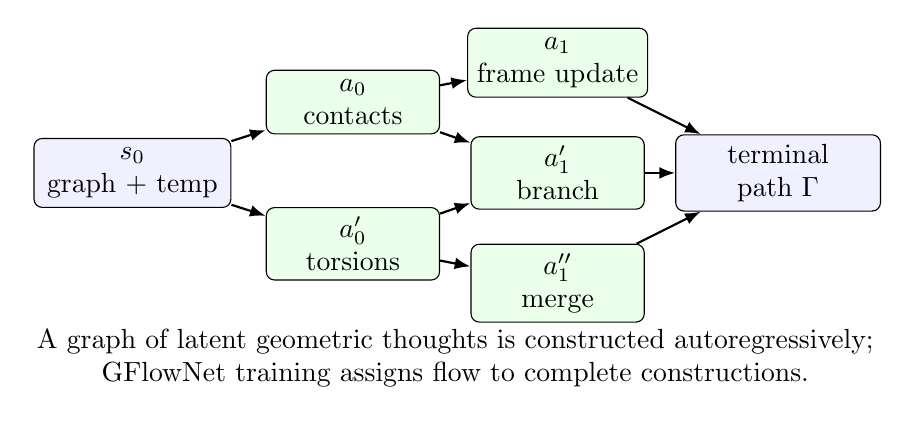
\begin{tikzpicture}[
  box/.style={draw,rounded corners=3pt,align=center,minimum height=8mm,fill=blue!6},
  small/.style={draw,rounded corners=3pt,align=center,minimum height=6mm,fill=green!8},
  arrow/.style={-{Latex[length=2mm]},thick}
]
\node[box,minimum width=2.5cm] (s0) at (0,0) {$s_0$\\graph + temp};
\node[small,minimum width=2.2cm] (a0) at (2.8,0.9) {$a_0$\\contacts};
\node[small,minimum width=2.2cm] (a1) at (2.8,-0.9) {$a_0'$\\torsions};
\node[small,minimum width=2.2cm] (b0) at (5.4,1.4) {$a_1$\\frame update};
\node[small,minimum width=2.2cm] (b1) at (5.4,0) {$a_1'$\\branch};
\node[small,minimum width=2.2cm] (b2) at (5.4,-1.4) {$a_1''$\\merge};
\node[box,minimum width=2.6cm] (term) at (8.2,0) {terminal\\path $\Gamma$};
\draw[arrow] (s0)--(a0);
\draw[arrow] (s0)--(a1);
\draw[arrow] (a0)--(b0);
\draw[arrow] (a0)--(b1);
\draw[arrow] (a1)--(b1);
\draw[arrow] (a1)--(b2);
\draw[arrow] (b0)--(term);
\draw[arrow] (b1)--(term);
\draw[arrow] (b2)--(term);
\node[align=center] at (4.1,-2.35) {A graph of latent geometric thoughts is constructed autoregressively;\\GFlowNet training assigns flow to complete constructions.};
\end{tikzpicture}
\caption{Graph-of-thought construction as a GFlowNet state graph. Branching preserves diverse hypotheses; merging lets compatible partial structures combine. The terminal object may be one conformation or a full trajectory.}
\label{fig:got}
\end{figure}

\section{Training Program}

\subsection{Stage 1: sequence and graph pretraining}

The first stage trains TokenGT without structure data in the strict run: no coordinate labels, no structure-token labels, no conformer libraries, no MD frames, and no structure-derived input features. It should include a sequence-linear-graph variant in which only ordered residue/base/atom tokens and nearest-neighbor polymer edges are visible. Objectives include:
\begin{enumerate}[leftmargin=2em]
  \item masked token reconstruction for residues, bases, atoms, and bond types;
  \item causal next-token or span prediction for autoregressive compatibility;
  \item graph denoising: corrupt atom types, bond orders, branches, or polymer edges and recover them;
  \item contrastive invariance under SMILES randomization, SELFIES alternatives, residue graph augmentations, and reverse-complement DNA where appropriate;
  \item masked edge prediction for covalent and syntactic edges;
  \item categorical Jacobian regularization to expose coupling maps.
\end{enumerate}

No coordinate or structure-token target is used, and no geometry-derived feature is inserted into the strict input. The goal is to learn biochemical syntax, grammar, co-occurrence, and functional priors, then test whether the sequence-linear graph alone is enough for oracle-guided structure-dynamics learning.

\subsection{Stage 2: latent geometry bootstrapping}

The second stage introduces latent geometry without supervised structures or external structure-derived features. In the sequence-linear-graph ablation, the model must generate contact hypotheses, hydrogen-bond hypotheses, distance constraints, torsions, and coordinate hypotheses from sequence embeddings and attention maps alone, then receive oracle feedback. Early training should begin with small systems to avoid impossible exploration.

A useful curriculum is:
\[
\begin{gathered}
\text{small rigid molecules}\to
\text{flexible small molecules}\to
\text{dipeptides}\to
\text{short peptides}\\
\to\text{single-domain mini-proteins}\to
\text{RNA hairpins}.
\end{gathered}
\]

For each system, the policy samples latent actions. The geometry decoder produces conformations. The oracle returns rewards. The GFlowNet objective updates the policy.

\subsection{Stage 3: trajectory rewards}

Once single-conformation sampling is stable, extend terminal objects from $X$ to $\Gamma=(X_0,\dots,X_K)$. The reward becomes:
\[
\log R_T(\Gamma)
=
-S_T(\Gamma)
-\lambda_{\mathrm{chem}}\sum_k \mathcal{V}_{\mathrm{chem}}(X_k)
-\lambda_{\mathrm{clash}}\sum_k \mathcal{V}_{\mathrm{clash}}(X_k)
-\lambda_{\mathrm{unc}}\sum_k u_{\mathrm{unc}}(X_k)
+r_{\mathrm{task}}(\Gamma).
\]
The path action $S_T$ should use oracle forces:
\[
S_T(\Gamma)=
\sum_{k=0}^{K-1}
\frac{
\left\|\Delta X_k+\Delta t M\nabla E_{\mathrm{eff}}(X_k)\right\|^2_{M^{-1}}
}{
4\Kb T\Delta t
}
\;+\;\alpha \sum_k \left|E_{\mathrm{eff}}(X_{k+1})-E_{\mathrm{eff}}(X_k)\right|_{\mathrm{barrier}}.
\]
The barrier term is optional and must be treated carefully, because real dynamics crosses barriers. Its role is to prevent huge unphysical jumps, not to prevent transitions.

\subsection{Stage 4: temperature calibration}

Temperature conditioning should be tested quantitatively:
\begin{enumerate}[leftmargin=2em]
  \item Does the energy distribution shift correctly with $\beta$?
  \item Does conformational diversity increase with $T$?
  \item Are low-temperature samples concentrated near low-energy basins?
  \item Does reweighting from $T_1$ to $T_2$ work over overlapping energy ranges?
  \item Does the learned path distribution satisfy approximate detailed balance?
\end{enumerate}

The model should receive $T$ through multiple mechanisms:
\[
h^{(0)}\leftarrow h^{(0)}+W_T\gamma(T),
\]
where $\gamma(T)$ is a Fourier or log-temperature embedding;
\[
\log R_T=-\beta E_{\mathrm{eff}}+\cdots;
\]
and
\[
\Sigma_k=\Sigma_\theta(s_k,T)
\]
for continuous action variance.

\section{Why Autoregressive Decoding Only Is Hard}

Diffusion and flow matching have become dominant in molecular generation because they naturally model continuous distributions. Autoregressive decoding is attractive because it aligns with TokenGT and graph-of-thought reasoning, but it faces three challenges.

\textbf{Long horizon.} A trajectory may require hundreds or thousands of time steps. Autoregressive error accumulation is severe. The model should generate at a coarse time scale first, then refine with conditional substeps.

\textbf{Continuous density.} GFlowNet trajectory balance requires log probabilities or log densities. The autoregressive head must have a tractable density, such as a Gaussian mixture or flow head.

\textbf{Physical reversibility.} Real equilibrium dynamics obeys detailed balance under appropriate conditions. A forward autoregressive generator can violate reversibility unless trained with backward policies, path rewards, or explicit reversibility checks.

The best compromise is hierarchical autoregression:
\[
\Gamma_{\mathrm{coarse}}
\sim p_\theta(\cdot|G,T),
\qquad
\Gamma_{\mathrm{fine}}
\sim p_\theta(\cdot|\Gamma_{\mathrm{coarse}},G,T).
\]
This remains autoregressive but avoids generating every femtosecond-scale step directly.

\section{Borrowable Ideas Without Violating the Constraint}

\subsection{From ESM3 and SLM}

Borrow:
\begin{enumerate}[leftmargin=2em]
  \item multiple tracks for sequence, graph, function, contacts, geometry, and confidence;
  \item iterative masked refinement as an auxiliary training mode, even if final decoding is autoregressive;
  \item compact local-structure abstractions, but learned as latent codebooks over model-proposed, oracle-scored hypotheses rather than from external structure datasets;
  \item promptable conditioning.
\end{enumerate}

Avoid in strict mode:
\begin{enumerate}[leftmargin=2em]
  \item supervised structure-token prediction from PDB or MD;
  \item training a VQ-VAE on known structures;
  \item using ESM3 structure tracks as target labels.
\end{enumerate}

\subsection{From BioEmu}

Borrow:
\begin{enumerate}[leftmargin=2em]
  \item the emphasis on equilibrium distributions rather than single structures;
  \item thermodynamic calibration;
  \item property-prediction fine-tuning ideas for scalar experimental observables;
  \item careful out-of-distribution benchmarks.
\end{enumerate}

Avoid in strict mode:
\begin{enumerate}[leftmargin=2em]
  \item MD data as training targets;
  \item AFDB/PDB structures as supervised conformational examples.
\end{enumerate}

Scalar experimental observables occupy a gray zone. If the rule forbids all structure data but permits non-structural experimental measurements, then stability, binding, or activity labels could be used in a PPFT-like way. If the rule is pure oracle-only, they should be reserved for evaluation.

\subsection{From flow matching and diffusion}

Borrow:
\begin{enumerate}[leftmargin=2em]
  \item continuous latent spaces;
  \item noise schedules as temperature-like curricula;
  \item coarse-to-fine refinement;
  \item score-like force matching against oracle gradients.
\end{enumerate}

Avoid:
\begin{enumerate}[leftmargin=2em]
  \item denoising supervision from ground-truth conformations;
  \item training on MD paths.
\end{enumerate}

There is still a way to use force information without structure data. If the model proposes $X$, the oracle gives $\nabla U(X)$. The model can train local update heads to align with oracle forces:
\[
\mathcal{L}_{\mathrm{force}}=
\left\|
g_\theta(X,G,T)+M\nabla E_{\mathrm{eff}}(X)
\right\|^2,
\]
where $g_\theta$ is the predicted drift. This is online oracle supervision, not trajectory-data supervision.

\subsection{From Boltzmann Generators}

Boltzmann Generators learn invertible maps from a simple prior to a Boltzmann distribution and can use energy-based losses plus reweighting \cite{noe2019boltzmann}. The proposed method can borrow:
\begin{enumerate}[leftmargin=2em]
  \item explicit density accounting;
  \item importance weights;
  \item free energy estimation;
  \item checks for effective sample size.
\end{enumerate}

The challenge is that invertible coordinate maps for large biomolecules are hard. GFlowNets may be more natural for compositional graph construction, but Boltzmann Generator diagnostics remain valuable.

\section{Oracle Design and UMA Caveats}

UMA is attractive because it is a universal model for atoms trained on a very large set of three-dimensional atomic structures across molecules, materials, and catalysts, with scaling-law analysis and mixture-of-linear-experts architecture \cite{wood2025uma}. It offers fast approximate energies and forces, which is exactly the kind of signal an oracle-guided generator needs.

However, using UMA directly as the sole biomolecular folding oracle is risky.

\begin{enumerate}[leftmargin=2em]
  \item \textbf{Solvent.} Protein folding and nucleic-acid structure are aqueous phenomena. Vacuum-like energies can favor collapsed or unrealistic states.
  \item \textbf{Ions and electrostatics.} RNA and DNA depend strongly on counterions and long-range electrostatics.
  \item \textbf{Temperature.} Many MLIPs predict potential energy surfaces, not finite-temperature free energies.
  \item \textbf{Domain of applicability.} Universal does not mean uniformly reliable for every biomolecular conformation, protonation state, or large charged complex.
  \item \textbf{Adversarial exploitation.} A generator trained to maximize oracle reward may find regions where the oracle is wrong.
\end{enumerate}

Therefore the oracle should be a wrapper:
\[
\begin{aligned}
\oracle = \big[&
\mathrm{UMA}
+ \mathrm{classical\ bonded\ terms}
+ \mathrm{implicit\ solvent}\\
&+ \mathrm{electrostatic\ correction}
+ \mathrm{validity\ filters}
+ \mathrm{uncertainty\ penalty}
\big].
\end{aligned}
\]
For early experiments, one can compare UMA with OpenMM force fields, xTB, ANI, MACE, or DFT for small systems. The point is not that UMA is guaranteed correct; it is that the architecture should accept an oracle interface and learn from it.

\section{Mathematical Specification of the Proposed Method}

\subsection{Conditioning object}

Let
\[
c=(G,\rho,T,\epsilon)
\]
where $G$ is the biomolecular graph, $\rho$ is resolution metadata, $T$ is physical temperature, and $\epsilon$ describes environment: pH, solvent model, ionic strength, ligand state, or membrane context.

\subsection{Policy}

The TokenGT encoder maps $G$ to embeddings:
\[
H_0=\tokgt_\theta(G).
\]
The autoregressive policy constructs a latent object $y$:
\[
p_\theta(y|c)=\prod_{k=1}^{K}p_\theta(a_k|s_k,c),
\qquad y=f(a_{1:K},c).
\]
$y$ may be a conformation latent or a path latent.

\subsection{Decoder}

The geometry decoder maps $y$ to a coordinate distribution:
\[
p_\eta(X|y,c)
\quad\text{or}\quad
p_\eta(\Gamma|y,c).
\]
In implementation this can be a deterministic solver plus stochastic perturbations:
\[
X=\operatorname{Solve}(y,c)+\epsilon_X,
\qquad \epsilon_X\sim q_\eta(\cdot|y,c).
\]

\subsection{Reward}

For terminal conformations:
\[
R_T(y)=
\E_{X\sim p_\eta(\cdot|y,c)}
\left[
\exp[-\beta E_{\mathrm{eff}}(X,c)]
\mathbf{1}_{\mathrm{valid}}(X,c)
\exp[-\lambda u_{\mathrm{unc}}(X)]
\right].
\]
For trajectories:
\[
R_T(y)=
\E_{\Gamma\sim p_\eta(\cdot|y,c)}
\left[
\exp[-S_T(\Gamma,c)]
\prod_k \mathbf{1}_{\mathrm{valid}}(X_k,c)
\exp[-\lambda\sum_k u_{\mathrm{unc}}(X_k)]
\right].
\]
Monte Carlo estimates are acceptable if variance is controlled.

\subsection{GFlowNet objective}

For a sampled construction trajectory $\tau=(s_0,\dots,s_n=y)$:
\[
\mathcal{L}_{\mathrm{TB}}(\theta)=
\left(
\log Z_\theta(c)
+\sum_{t=0}^{n-1}\log p_F(a_t|s_t,c)
-\sum_{t=0}^{n-1}\log p_B(a_t^-|s_{t+1},c)
-\log R_T(y)
\right)^2.
\]
The conditioning object $c$ may have its own partition estimate $Z_\theta(c)$. If training across many molecules and temperatures, one can use a learned partition network:
\[
\log Z_\theta(c)=z_\theta(\operatorname{pool}(H_0),\gamma(T),\epsilon).
\]

\subsection{Force regularization}

For online oracle queries, add a local force consistency term:
\[
\mathcal{L}_{\mathrm{drift}}
=
\sum_{k}
\left\|
\mu_\theta(s_k,T)
+\Delta t\,M\nabla E_{\mathrm{eff}}(X_k)
\right\|^2,
\]
where $\mu_\theta$ is the mean predicted coordinate or latent update translated into coordinate space. This encourages proposals to respect local physics.

\subsection{Detailed balance diagnostic}

For generated transitions $X\to X'$, test:
\[
\Delta_{\mathrm{DB}}(X,X')=
\log \hat{p}_\theta(X'|X)
-\log \hat{p}_\theta(X|X')
+\beta\left(E_{\mathrm{eff}}(X')-E_{\mathrm{eff}}(X)\right).
\]
At equilibrium, $\Delta_{\mathrm{DB}}$ should be near zero in distribution for reversible dynamics. This is a diagnostic, not necessarily a training loss in the first version.

\section{Minimum Viable Algorithm}

The simplest executable version should not begin with proteins. It should begin with a small-molecule conformer task where the graph is known, torsional degrees of freedom are clear, and oracle calls are cheap. The algorithm below is deliberately modest: it is the smallest version that tests the central claim that GFlowNet training from oracle rewards can produce a diverse temperature-conditioned sampler without training on conformer data.

\begin{center}
\begin{minipage}{0.93\linewidth}
\textbf{Algorithm 1: Oracle-amortized TokenGT-GFlowNet conformer sampler}
\begin{enumerate}[leftmargin=2em]
  \item Parse a SMILES or SELFIES string into an atom-bond graph $G$.
  \item Build TokenGT tokens: one token per atom and one token per bond, with spectral graph encodings and bond-type features.
  \item Encode $G$ with TokenGT to obtain graph context $H_0$.
  \item Initialize a GFlowNet state $s_0=(G,T,H_0,\emptyset)$.
  \item Autoregressively sample continuous torsion actions $a_k\sim p_F(a_k|s_k,T)$ until all rotatable bonds and optional refinement actions are assigned.
  \item Reconstruct a conformation $X$ from the molecular graph and torsions, then repair local geometry with a constrained optimizer.
  \item Query the oracle for energy, validity, forces, and uncertainty:
  \[
  (\hat{E},\hat{F},u_{\mathrm{unc}},v_{\mathrm{chem}})=\oracle(X,G,T).
  \]
  \item Compute
  \[
  \log R_T(X)=
  -\beta E_{\mathrm{eff}}(X)
  -\lambda_{\mathrm{unc}}u_{\mathrm{unc}}(X)
  -\lambda_{\mathrm{chem}}v_{\mathrm{chem}}(X).
  \]
  \item Update the forward policy, backward policy, and partition estimator with trajectory balance.
  \item Add $(G,T,X,R_T,\oracle\text{-metadata})$ to replay.
  \item Periodically rescore a sample subset with an independent oracle and report oracle exploitation rate.
\end{enumerate}
\end{minipage}
\end{center}

This algorithm tests the method in a domain where success is not ambiguous. If the GFlowNet is working, it should recover multiple conformer basins in reward-proportional frequencies. If a reward-maximizing RL baseline collapses to one low-energy basin while the GFlowNet covers several thermally accessible basins, that is direct evidence for the distributional value of GFlowNets. If both collapse, the reward scaling, action parameterization, or replay strategy is broken.

The protein version differs mainly in the coordinate decoder. Torsions become backbone, side-chain, and local-frame variables; the oracle wrapper becomes more elaborate; and the reward shifts from terminal conformer energy to a mixture of conformation and path-action terms. The training logic remains the same.

\section{Implementation Plan}

\subsection{Phase 0: reproducibility scaffold}

Create a codebase with:
\begin{enumerate}[leftmargin=2em]
  \item graph parsers for FASTA, SMILES, SELFIES, and RNA/DNA;
  \item a $\bioselfies$ parser/decoder that maps proteins, nucleic acids, glycans, ligands, modifications, and complexes to typed graphs;
  \item a hybrid multiresolution tokenizer with residue/base tokens, ligand SELFIES tokens, side-chain torsion heads, nucleic-acid torsion heads, and adaptive all-atom patches;
  \item hydrogen-bond typing utilities for donors, acceptors, implicit hydrogens, protonation states, and canonical base-pair H-bond patterns;
  \item RDKit integration for small molecules;
  \item Biopython or equivalent parsers for biomolecular sequences;
  \item TokenGT-compatible graph batching;
  \item oracle interface abstraction;
  \item replay buffer for generated candidates;
  \item experiment registry with molecule, temperature, oracle, and reward versioning.
\end{enumerate}

Every oracle call should be logged. Without logging, the project will not be scientifically interpretable.

\subsection{Current UGM implementation status}

The accompanying repository implements a first executable version of the strict symbolic-input path. The implemented \(\bioselfies\) layer is a total decoder for a supported bracket grammar:
\[
[AA:x],\ [DNA:x],\ [RNA:x],\ [ATOM:x],\ [LINK:x],\ [MOD:x],
\]
together with SELFIES atom tokens, chain breaks, branch controls, adaptive patch controls, hydrogen-bond controls, torsion controls, and latent-thought controls. Unknown records are preserved as explicit unknown nodes rather than rejected. The decoder produces typed graph nodes and edges plus vocabulary records such as \texttt{BIOSELFIES:[AA:A]}, \texttt{HYBRID:atom\_patch}, \texttt{HBOND:candidate}, and \texttt{TORSION:sidechain\_chi}. It does not create coordinate, distance, energy, force, PDB, mmCIF, SDF, conformer, or trajectory labels.

The current coordinate path is also implemented as an oracle-feedback path rather than a supervised structure path. Source-side \texttt{UMA\_COORD\_QUERY:*} records are derived from symbolic molecule or sequence records; for protein \(\bioselfies\) records, the query generator uses a coarse backbone pattern \((N,C,C,O)\) per residue. A gated coordinate head reads continuous positions from the same hidden graph-of-thought embeddings that drive graph-token decoding. UMA/FairChem then scores the generated candidate coordinates at the graph's Kelvin temperature and returns detached forces. The training surrogate
\[
\mathcal{L}_{\mathrm{UMA\text{-}coord}}
=-\frac{1}{n}\sum_i \langle \operatorname{sg}(F_i^{\mathrm{UMA}}),x_i\rangle
+\lambda_{\mathrm{center}}\mathcal{L}_{\mathrm{center}}
+\lambda_{\mathrm{repel}}\mathcal{L}_{\mathrm{repel}}
\]
backpropagates only through the model's coordinate readout and hidden state. With multiple oracle rollout steps, the generated coordinates are updated by detached UMA forces before rescoring, so repeated graph-of-thought iterations act like a short physical-time discretization. The implementation therefore matches the paper's boundary: no direct structure labels are copied, but physical information enters through the oracle.

\subsection{Phase 1: small-molecule proof of principle}

Start with small molecules because the method can fail cheaply. Use SELFIES or SMILES corpora for pretraining. Parse to atom-bond graphs. Generate torsion vectors. Use RDKit ETKDG and force-field minimization as baselines. Use UMA, MMFF, xTB, or ANI-like potentials for rewards.

Tasks:
\begin{enumerate}[leftmargin=2em]
  \item sample conformers for small molecules with known conformer ensembles;
  \item estimate energy histograms at multiple temperatures;
  \item test mode coverage against GEOM-like evaluation sets, but do not train on those conformers;
  \item test reweighting between temperatures.
\end{enumerate}

Metrics:
\[
\mathrm{COV},\quad \mathrm{MAT},\quad
\Delta E,\quad
\mathrm{ESS},\quad
\mathrm{validity},\quad
\mathrm{diversity},\quad
\mathrm{oracle\ exploit\ rate}.
\]

\subsection{Phase 2: peptides and toy proteins}

Move to alanine dipeptide, short peptides, and miniproteins. Use internal coordinates. In the strict run, use Ramachandran distributions only for evaluation, never as training priors. The oracle should include solvent corrections. Evaluate against MD only as held-out validation.

Tasks:
\begin{enumerate}[leftmargin=2em]
  \item recover alanine dipeptide basins in $(\phi,\psi)$;
  \item sample peptide conformers at multiple temperatures;
  \item generate coarse trajectories between basins;
  \item compare path action to short MD rollouts.
\end{enumerate}

\subsection{Phase 3: protein monomers}

For proteins, begin with residue-level generation and reconstruct all atoms afterward. Use sequence-only pretraining on UniRef/UniProt-like corpora. The first protein run should be the sequence-linear graph: residue nodes and polymer-neighbor edges only. Candidate non-covalent edge tokens can be proposed by attention/Jacobian heads, scored by the oracle, and promoted into later graph-of-thought states, but they should not be supplied from structure.

Evaluation datasets may include DESRES fast folders, ATLAS, BPTI, IDPs, and known conformational change pairs, but only for evaluation. Compare against BioEmu, AlphaFlow, SLM, DynaFold, MDGen, ESMFold/AlphaFold sampling, and classical MD.

Metrics:
\begin{enumerate}[leftmargin=2em]
  \item contact precision against known structures;
  \item RMSD/TM-score coverage of known conformers;
  \item free energy basin occupancy;
  \item Jensen-Shannon divergence of torsion distributions;
  \item path plausibility and barrier crossing;
  \item detailed balance residuals;
  \item stability of generated structures under short MD relaxation.
\end{enumerate}

\subsection{Phase 4: nucleic acids}

RNA and DNA should be introduced only after the protein and small-molecule loops are stable. Use RNAcentral and genomic corpora for pretraining. Generate base-pair, stacking, sugar pucker, and backbone torsion hypotheses. Compare to RhoFold+, classical secondary structure models, and held-out RNA structures.

Key tests:
\begin{enumerate}[leftmargin=2em]
  \item RNA hairpin folding;
  \item duplex stability at different temperatures;
  \item base-pair opening events;
  \item ion-sensitive motifs in simplified environments.
\end{enumerate}

\subsection{Phase 5: complexes}

Only then attempt protein-ligand, protein-RNA, protein-DNA, or protein-protein systems. The token count and oracle burden rise sharply. The first complex experiments should be local: generate ligand conformations in a fixed pocket, or generate side-chain rearrangements near a ligand.

\section{Benchmark Plan}

\subsection{Method families to compare}

The comparison should include:
\begin{enumerate}[leftmargin=2em]
  \item TokenGT-GFN oracle sampler variants, including sequence-linear-graph and enriched-graph inputs;
  \item TokenGT trained with standard RL-style reward maximization;
  \item TokenGT autoregressive sampler without GFlowNet;
  \item Boltzmann Generator or normalizing-flow baselines for small systems;
  \item RDKit ETKDG / force-field baselines for small molecules;
  \item MD baselines using the same oracle or a classical force field;
  \item BioEmu, AlphaFlow, P2DFlow, SLM, DynaFold, and MDGen where applicable;
  \item structure predictors with sampling tricks, such as MSA subsampling or dropout, where applicable.
\end{enumerate}

The key scientific comparison is not just accuracy. It is the tradeoff between:
\[
\text{training data used},\quad
\text{oracle calls},\quad
\text{compute},\quad
\text{physical fidelity},\quad
\text{mode coverage}.
\]

\subsection{Ablations}

Essential ablations:
\begin{enumerate}[leftmargin=2em]
  \item sequence-only linear graph versus enriched non-structural biomolecular graphs;
  \item native FASTA/SMILES/graph inputs versus $\bioselfies$-only inputs;
  \item all-$\bioselfies$ tokenization versus hybrid multiresolution tokenization;
  \item full all-atom tokens versus adaptive all-atom patches at ligand and nucleic-acid interfaces;
  \item remove edge tokens;
  \item remove spectral positional encodings;
  \item replace GFlowNet with reward-weighted maximum likelihood;
  \item replace GFlowNet with PPO or another RL objective;
  \item remove force regularization;
  \item remove uncertainty penalties;
  \item disable attention/contact calibration;
  \item use terminal energy reward only versus path-action reward;
  \item fix sampling temperature versus learned temperature calibration.
\end{enumerate}

\subsection{Success criteria}

The proposal should be considered promising only if it achieves all of the following on small systems:
\begin{enumerate}[leftmargin=2em]
  \item valid chemistry above 99\% for small molecules and peptides;
  \item non-collapsed mode coverage under multimodal energy landscapes;
  \item energy distributions that respond correctly to $T$;
  \item no obvious oracle exploitation under independent oracle checks;
  \item better sample efficiency than naive random conformer search;
  \item stronger diversity than RL maximization at comparable reward.
\end{enumerate}

For proteins, success is more modest at first:
\begin{enumerate}[leftmargin=2em]
  \item plausible local geometry;
  \item stable short MD relaxation;
  \item partial recovery of known conformational basins;
  \item meaningful temperature-dependent diversity;
  \item improved coverage over sequence-only static predictors with dropout.
\end{enumerate}

\section{Failure Modes}

\subsection{Oracle exploitation}

The generator may find conformations that UMA scores as low energy but are physically wrong. This is common in learned reward systems. Mitigations:
\begin{enumerate}[leftmargin=2em]
  \item uncertainty penalties;
  \item ensemble of oracles;
  \item periodic high-fidelity rescoring;
  \item adversarial validation sets;
  \item conservative trust regions in latent space;
  \item replay buffer filtering.
\end{enumerate}

\subsection{Entropy collapse}

Even though GFlowNets are designed for diverse sampling, poor reward scaling can still collapse modes. Use log-reward normalization, temperature sweeps, replay buffers, and explicit partition estimation diagnostics.

\subsection{Invalid geometry}

Continuous latent generation may produce impossible distances or torsions. The geometry decoder should enforce hard chemistry before oracle scoring. For proteins, use internal coordinate reconstruction and side-chain packing. For small molecules, use valence-aware RDKit graphs. For nucleic acids, enforce sugar-phosphate backbone constraints.

\subsection{Kinetic hallucination}

A sequence of low-energy conformations is not a trajectory. To claim dynamics, the model must satisfy path-level checks: transition probabilities, time correlations, approximate detailed balance, realistic barrier crossings, and stability under MD refinement.

\subsection{Temperature miscalibration}

The model sampling temperature can masquerade as physical temperature. Calibration must be empirical. Reweighting tests and energy fluctuation identities should be part of every benchmark.

\section{A Pragmatic Research Roadmap}

\subsection{Six-month version}

\begin{enumerate}[leftmargin=2em]
  \item Implement TokenGT-style atom-bond and residue graph encoder.
  \item Pretrain on SELFIES/SMILES and small protein sequences.
  \item Build continuous torsion decoder for small molecules.
  \item Train GFlowNet sampler with MMFF/xTB/UMA reward.
  \item Benchmark conformer generation and temperature response.
\end{enumerate}

\subsection{Twelve-month version}

\begin{enumerate}[leftmargin=2em]
  \item Add peptide internal-coordinate decoder.
  \item Add force regularization and path-action rewards.
  \item Test alanine dipeptide, short peptides, and mini-proteins.
  \item Compare to MD and learned conformer baselines.
  \item Publish the small-system oracle-amortized GFlowNet result.
\end{enumerate}

\subsection{Twenty-four-month version}

\begin{enumerate}[leftmargin=2em]
  \item Scale to proteins with residue-level TokenGT and all-atom reconstruction.
  \item Add nucleic-acid tokenizer and simplified RNA hairpin experiments.
  \item Integrate UMA with solvent/electrostatic correction.
  \item Evaluate against BioEmu, AlphaFlow, DynaFold, and MDGen on held-out tasks.
  \item Release a benchmark suite for structure-data-free oracle learning, with a separately labeled geometry-feature ablation track.
\end{enumerate}

\section{Position Relative to NeurIPS-Level Novelty}

The paper-worthy novelty is not simply ``use TokenGT for molecules.'' That is plausible but incremental. The stronger contribution would be:
\begin{enumerate}[leftmargin=2em]
  \item a formalization of biomolecular dynamics generation as a GFlowNet over latent graph-of-thought constructions;
  \item an oracle-only, no-demonstration training setting for molecular conformational distributions;
  \item a continuous autoregressive alternative to diffusion/flow matching for molecular trajectories;
  \item a careful thermodynamic reward design linking GFlowNet terminal sampling to Boltzmann and path distributions;
  \item a benchmark showing when oracle-amortized learning can compete with data-driven dynamics models.
\end{enumerate}

A NeurIPS-quality version needs rigorous negative results too. If the method fails on protein folding but succeeds on small-molecule conformers, that is still valuable. If it works only with a hybrid oracle rather than UMA alone, that is important. If GFlowNets beat RL on diversity but not on energy, that is a publishable insight. The field needs honest maps of where data-free oracle training breaks.

\section{Concluding View}

The proposed system is scientifically sound only if framed carefully. TokenGT provides a graph-native Transformer substrate. Protein LMs and gLM2 show that sequence and context training can induce structural couplings. GFlowNets provide a principled alternative to reward maximization by sampling proportional to reward. UMA-like MLIPs provide scalable physical feedback. Attention maps can seed contact hypotheses, especially when edge tokens make relations first-class. Together, these ingredients support a plausible research program.

But there is no free lunch. Sequence and graph syntax alone do not determine molecular dynamics without feedback. The oracle is the physics. The model's job is to learn structure-dynamics from sequence-only or graph-augmented inputs by amortizing oracle-guided sampling, not to replace physical grounding. The most rigorous path is to start with small molecules, prove temperature-calibrated Boltzmann sampling under oracle rewards, extend to sequence-linear peptides with path-action rewards, measure what enriched graph inputs add, and only then attempt proteins, nucleic acids, and complexes.

If successful, the result would occupy a distinctive niche between classical MD, structure-trained diffusion models, and sequence-only language models: an autoregressive graph reasoning model that learns physical distributions through reward-proportional oracle feedback, with no direct structure training examples.

\appendix
\newpage
\section{Extended Mathematical Notes}

\subsection{Euclidean distance geometry}

Given a complete distance matrix $D$ with entries $d_{ij}$, define the squared distance matrix $D^{(2)}$. A centered Gram matrix is
\[
B=-\frac{1}{2}JD^{(2)}J,
\qquad
J=I-\frac{1}{N}\mathbf{1}\mathbf{1}^\top.
\]
The distances are embeddable in $\R^3$ if $B\succeq 0$ and $\operatorname{rank}(B)\le 3$. For sparse noisy distances, one solves a constrained optimization problem. The TokenGT model should output uncertainty-weighted sparse distances, not necessarily a complete matrix.

\subsection{Internal coordinate reconstruction}

For a polymer, a new atom position can be reconstructed from three previous atoms using bond length $r$, bond angle $\theta$, and dihedral $\phi$. This makes it natural for the model to generate torsions while keeping local covalent geometry fixed. Proteins can use backbone torsions $(\phi,\psi,\omega)$ plus side-chain torsions $\chi_i$. RNA requires a richer torsion set.

\subsection{Path ensembles}

For transition paths from basin $A$ to basin $B$, one can condition on
\[
X_0\in A,\qquad X_K\in B,\qquad X_k\notin A\cup B\;\;0<k<K.
\]
The reward becomes
\[
R(\Gamma)\propto
\exp[-S_T(\Gamma)]
\mathbf{1}\{X_0\in A,X_K\in B\}
\prod_{k=1}^{K-1}\mathbf{1}\{X_k\notin A\cup B\}.
\]
This is closer to transition path sampling than equilibrium sampling. It should be benchmarked separately.

\subsection{Partition functions and free energies}

If a GFlowNet estimates $Z_\theta(c)$, then
\[
F(c,T)=-\beta^{-1}\log Z(c)
\]
is a free energy estimate under the reward-defined ensemble. This is one of the most attractive reasons to use GFlowNets. However, $Z_\theta$ is only as meaningful as the reward and state space.

\section{Detailed Experimental Matrix}

\begingroup
\small
\setlength{\tabcolsep}{3pt}
\begin{longtable}{p{0.13\linewidth}p{0.17\linewidth}p{0.17\linewidth}p{0.18\linewidth}p{0.17\linewidth}}
\caption{Proposed benchmark matrix. In the strict run, training data allowed means non-structural sequence or graph corpora only; all listed structural or trajectory datasets are held out for evaluation, calibration diagnostics, or baseline comparison.}\\
\toprule
Domain & Training data allowed & Oracle & Evaluation data & Primary question\\
\midrule
\endfirsthead
\toprule
Domain & Training data allowed & Oracle & Evaluation data & Primary question\\
\midrule
\endhead
Toy potentials & none beyond potential queries & analytic double wells, Muller-Brown & exact samples / MCMC & Does GFN learn proportional sampling?\\
Sequence-linear peptides & FASTA only, polymer-neighbor edges only & UMA/OpenMM hybrid & MD and known basins held out & Does sequence-only input learn structure-dynamics?\\
BioSELFIES universal input & $\bioselfies$ strings only & UMA/hybrid oracle & native parser and held-out structure/dynamics benchmarks & Does robust universal serialization preserve useful information?\\
Hybrid protein-ligand tokenization & protein sequence plus ligand SELFIES, no structure targets & UMA/hybrid + solvent & docking, side-chain, and MD benchmarks held out & Does adaptive all-atom patching preserve interface physics efficiently?\\
Small molecules & SMILES/SELFIES only & MMFF, xTB, UMA, DFT subset & GEOM / QM9 conformers held out & Can it cover conformer modes?\\
Alanine dipeptide & sequence and chemistry only & OpenMM/UMA hybrid & long MD free energy surface & Does it recover Ramachandran basins?\\
Peptides & FASTA only & OpenMM/UMA hybrid & DESRES/short MD held out & Does path reward improve trajectories?\\
Proteins & sequence corpora only & UMA/hybrid + solvent & BPTI, ATLAS, conformer pairs & Does it generate plausible ensembles?\\
RNA motifs & RNA sequence corpora only & RNA force field / hybrid & PDB/RNA-Puzzles held out & Does graph tokenization help sparse data?\\
Complexes & sequences and ligand graphs only & hybrid oracle & docking/complex benchmarks held out & Can it handle typed biomolecular graphs?\\
\bottomrule
\end{longtable}
\endgroup

\section{Ablation Details}

\subsection{GFlowNet versus RL}

For the same reward, compare:
\[
\max_\theta \E_{p_\theta}[\log R(X)]
\]
against GFlowNet trajectory balance. The expected reward objective should find high-reward modes but may ignore lower-reward modes with meaningful Boltzmann probability. The GFlowNet should better approximate the full reward-proportional distribution.

\subsection{Terminal reward versus path reward}

A terminal reward
\[
R(X_K)=\exp[-\beta E(X_K)]
\]
can produce good endpoints but unphysical transitions. A path reward
\[
R(\Gamma)=\exp[-S_T(\Gamma)]
\]
penalizes implausible jumps. Benchmark both. This ablation is essential for distinguishing ensemble generation from trajectory generation.

\subsection{Sequence-linear graph versus enriched graph}

The cleanest representation ablation is:
\[
G_{\mathrm{lin}}
\quad\text{vs.}\quad
G_{\mathrm{chem}}
\quad\text{vs.}\quad
G_{\mathrm{context}}
\quad\text{vs.}\quad
G_{\mathrm{self}\text{-}\mathrm{proposed}}.
\]
All variants must use the same training sequences, the same oracle, the same reward, and the same oracle-call budget. The linear graph receives only ordered tokens and neighbor edges. The enriched graphs add non-structural chemistry, biological context, or model-proposed interaction edges. A positive result for $G_{\mathrm{lin}}$ would support the strongest claim: TokenGT can learn structure-dynamics from sequence-only inputs through UMA scoring, attention contacts, and embedding geometry. A positive gap for enriched graphs would show that additional biomolecular graph information adds useful inductive bias rather than merely decorative complexity.

\subsection{Edge tokens}

Remove edge tokens and feed only vertex tokens with adjacency-derived biases. If performance drops on long-range contacts, ligand constraints, base pairing, or torsion compatibility, that supports the TokenGT-specific hypothesis.

\subsection{Geometry-feature tokens}

Run the strict model and a geometry-feature model under matched oracle budgets. The strict model receives only sequence, graph, grammar, temperature, and oracle feedback. The geometry-feature ablation additionally receives distances, angles, torsions, local frames, contact probabilities, or orientation descriptors as vertex and edge features. Report the provenance of those features explicitly:
\[
\text{oracle-generated}
\quad\text{vs.}\quad
\text{physics-initialized}
\quad\text{vs.}\quad
\text{database-derived}.
\]
The first two variants test whether online physics helps TokenGT organize its latent space; the third tests an upper bound under extra structural information. None of these ablations should be pooled with the strict no-structure-data result.

\section{Falsification Tests and Decision Rules}

A research program of this kind needs predefined failure criteria. Otherwise every failure can be redescribed as a need for more scale. The following tests should be run before any large protein claim.

\subsection{Test 1: oracle proportionality on toy systems}

Use analytic potentials with known or high-accuracy reference distributions. Train the GFlowNet only through oracle queries. Estimate the terminal density and compare it to $\pi_\beta(x)\propto\exp[-\beta U(x)]$ by KL divergence, Wasserstein distance, and basin probabilities. If the sampler cannot learn toy Boltzmann distributions, the method is not ready for molecules.

\subsection{Test 2: small-molecule mode coverage}

On held-out small molecules, compare against RDKit ETKDG, torsion random search, and a reward-maximizing RL baseline. The decision rule should be:
\[
\text{pass if}\quad
\mathrm{coverage}_{\mathrm{GFN}}>\mathrm{coverage}_{\mathrm{RL}}
\quad\text{at matched oracle budget and validity}.
\]
If GFlowNet training does not improve diversity at fixed reward quality, its main rationale is weakened.

\subsection{Test 3: temperature monotonicity}

For each molecule or peptide, evaluate at $T_1<T_2<T_3$. The entropy of sampled conformational basins and the mean energy should generally increase with $T$, while low-temperature samples should concentrate in low-energy basins. Violations indicate that model sampling temperature has replaced physical temperature.

\subsection{Test 4: independent-oracle agreement}

Rescore generated samples with a second oracle. A high fraction of samples whose primary-oracle energy is excellent but independent-oracle energy is poor indicates reward hacking. The project should report this as an oracle failure, not as a model success.

\subsection{Test 5: path realism}

For trajectory claims, compare generated transitions to short unbiased or restrained MD rollouts initialized from generated frames. Passing endpoint tests is insufficient. A trajectory model must produce finite step sizes, plausible force-aligned drifts, approximate detailed-balance residuals, and stable short relaxations.

\subsection{Decision rules}

The program should branch based on results:
\begin{enumerate}[leftmargin=2em]
  \item If toy and small-molecule tests fail, fix the GFlowNet and action space before scaling.
  \item If small molecules pass but peptides fail, improve geometry decoding and solvent corrections.
  \item If peptides pass but proteins fail, introduce hierarchical residue-to-atom generation and stronger uncertainty penalties.
  \item If all domains show oracle exploitation, the oracle wrapper is the bottleneck.
  \item If equilibrium samples work but paths fail, publish the method as an ensemble sampler and defer dynamics claims.
\end{enumerate}

\section{Practical Token Schemas}

\subsection{Protein residue graph}

Node features:
\[
\begin{gathered}
\text{amino acid},\text{chain id},\text{residue index},\\
\text{modification},\text{mask flag}.
\end{gathered}
\]
Edge features:
\[
\begin{gathered}
\text{polymer adjacency},\text{disulfide candidate},\text{same-chain},\\
\text{different-chain},\text{latent contact candidate},
\text{H-bond candidate},\\
\text{confidence}.
\end{gathered}
\]

\subsection{Small molecule atom graph}

Node features:
\[
\begin{gathered}
\text{element},\text{formal charge},\text{aromaticity},\text{hybridization},\\
\text{chirality},\text{implicit H count},
\text{H-bond donor},\text{H-bond acceptor}.
\end{gathered}
\]
Edge features:
\[
\text{bond order},\text{aromatic},\text{ring},\text{stereo},\text{rotatable}.
\]

\subsection{Protein-ligand hybrid graph}

Coarse protein tokens:
\[
\begin{gathered}
\text{residue},\text{chain},\text{backbone torsion head},\\
\text{side-chain torsion head},\text{patch flag}.
\end{gathered}
\]
Ligand tokens:
\[
\begin{gathered}
\text{SELFIES token},\text{atom token},\text{bond token},\\
\text{rotatable bond},\text{formal charge}.
\end{gathered}
\]
Interface edge features:
\[
\begin{gathered}
\text{hydrogen-bond candidate},\text{salt bridge candidate},
\text{hydrophobe contact},\\
\pi\text{-stacking},\text{metal coordination},\text{clash risk},\\
\text{donor/acceptor role},\text{H-bond geometry},
\text{oracle confidence}.
\end{gathered}
\]
Adaptive patch features:
\[
\begin{gathered}
\text{opened atom},\text{parent residue/base},\text{local frame},\\
\text{patch radius},\text{active torsion}.
\end{gathered}
\]

\subsection{Nucleic acid graph}

Node features:
\[
\text{base},\text{sugar},\text{phosphate},\text{chain id},\text{modification}.
\]
Edge features:
\[
\begin{gathered}
\text{backbone},\text{base pair candidate},\text{H-bond candidate},\\
\text{stacking candidate},\text{tertiary contact candidate}.
\end{gathered}
\]

\subsection{Nucleic-acid hybrid graph}

Coarse node features:
\[
\begin{gathered}
\text{base},\text{sugar},\text{phosphate},\text{strand id},\\
\text{sugar pucker head},\text{glycosidic torsion head}.
\end{gathered}
\]
Backbone action features:
\[
\alpha,\beta,\gamma,\delta,\epsilon,\zeta,\chi,p.
\]
Interaction edge features:
\[
\begin{gathered}
\text{Watson-Crick candidate},\text{wobble candidate},
\text{noncanonical pair},\\
\text{base-pair H-bond},\text{sugar-edge H-bond},\\
\text{base stacking},\text{ion bridge},\text{protein contact},
\text{ligand contact}.
\end{gathered}
\]

\section{Reference Implementation Sketch}

\begin{enumerate}[leftmargin=2em]
  \item Use PyTorch Geometric or custom batching to produce TokenGT token arrays.
  \item Store vertex tokens and edge tokens in a single sequence with segment IDs.
  \item Use spectral encodings with sign augmentation.
  \item Use a causal Transformer decoder over thought steps, cross-attending to encoded graph tokens.
  \item Parameterize continuous actions with Gaussian mixture heads.
  \item Decode small-molecule torsions first.
  \item Use an oracle queue with asynchronous scoring.
  \item Train with trajectory balance and replay.
  \item Log every sample, reward component, oracle version, and random seed.
\end{enumerate}

\section{Ethical and Scientific Reporting}

The method should not be marketed as replacing MD or experimental structure biology. It should be reported as an oracle-amortized proposal generator. Generated trajectories should be labeled by the oracle and environment used. If the oracle is UMA in vacuum, the results are UMA-vacuum trajectories, not biological reality. If an implicit solvent correction is used, it should be specified. For drug discovery, generated conformations must be validated by independent simulation and experiment.

\newpage
\begin{thebibliography}{99}

\bibitem{kim2022tokengt}
Jinwoo Kim, Tien Dat Nguyen, Seonwoo Min, Sungjun Cho, Moontae Lee, Honglak Lee, and Seunghoon Hong.
\newblock Pure Transformers are Powerful Graph Learners.
\newblock \emph{arXiv:2207.02505}, 2022.
\newblock \url{https://arxiv.org/abs/2207.02505}.

\bibitem{bengio2021gflownet}
Emmanuel Bengio, Moksh Jain, Maksym Korablyov, Doina Precup, and Yoshua Bengio.
\newblock Flow Network Based Generative Models for Non-Iterative Diverse Candidate Generation.
\newblock \emph{NeurIPS}, 2021.
\newblock \url{https://proceedings.neurips.cc/paper/2021/file/e614f646836aaed9f89ce58e837e2310-Paper.pdf}.

\bibitem{bengio2023gflownet}
Yoshua Bengio, Salem Lahlou, Tristan Deleu, Edward J. Hu, Mo Tiwari, and Emmanuel Bengio.
\newblock GFlowNet Foundations.
\newblock \emph{Journal of Machine Learning Research}, 24(210):1--55, 2023.
\newblock \url{https://www.jmlr.org/papers/v24/22-0364.html}.

\bibitem{malkin2022trajectory}
Nikolay Malkin, Moksh Jain, Emmanuel Bengio, Chen Sun, and Yoshua Bengio.
\newblock Trajectory Balance: Improved Credit Assignment in GFlowNets.
\newblock \emph{NeurIPS}, 2022.
\newblock \url{https://arxiv.org/abs/2201.13259}.

\bibitem{lu2025slm}
Jiarui Lu, Xiaoyin Chen, Stephen Zhewen Lu, Chence Shi, Hongyu Guo, Yoshua Bengio, and Jian Tang.
\newblock Structure Language Models for Protein Conformation Generation.
\newblock \emph{ICLR}, 2025.
\newblock \url{https://arxiv.org/abs/2410.18403}.

\bibitem{fan2025dynafold}
Zirui Fan, Junjie Zhu, and Hai-Feng Chen.
\newblock DynaFold: A Latent Diffusion Based Generative Framework for Protein Dynamic Trajectory.
\newblock \emph{bioRxiv}, 2025.
\newblock \url{https://www.biorxiv.org/content/10.1101/2025.09.14.676071v2}.

\bibitem{sengar2025ldfpg}
Aditya Sengar, Ali Hariri, Daniel Probst, Patrick Barth, and Pierre Vandergheynst.
\newblock Generative Modeling of Full-Atom Protein Conformations using Latent Diffusion on Graph Embeddings.
\newblock \emph{arXiv:2506.17064}, 2025.
\newblock \url{https://arxiv.org/html/2506.17064v1}.

\bibitem{hayes2024esm3}
Thomas Hayes, Roshan Rao, Halil Akin, Nicholas James Sofroniew, Deniz Oktay, Zeming Lin, Robert Verkuil, Vincent Quy Tran, and others.
\newblock Simulating 500 Million Years of Evolution with a Language Model.
\newblock \emph{bioRxiv}, 2024.
\newblock \url{https://doi.org/10.1101/2024.07.01.600583}.

\bibitem{cornman2024omg}
Andre Cornman, Jacob West-Roberts, Antonio Pedro Camargo, Simon Roux, Martin Beracochea, Milot Mirdita, Sergey Ovchinnikov, and Yunha Hwang.
\newblock The OMG Dataset: An Open MetaGenomic Corpus for Mixed-Modality Genomic Language Modeling.
\newblock \emph{bioRxiv}, 2024.
\newblock \url{https://doi.org/10.1101/2024.08.14.607850}.

\bibitem{vig2021bertology}
Jesse Vig, Ali Madani, Lav R. Varshney, Caiming Xiong, Richard Socher, and Nazneen Fatema Rajani.
\newblock BERTology Meets Biology: Interpreting Attention in Protein Language Models.
\newblock \emph{ICLR}, 2021.
\newblock \url{https://arxiv.org/abs/2006.15222}.

\bibitem{rao2021unsupervised}
Roshan M. Rao, Joshua Meier, Tom Sercu, Sergey Ovchinnikov, and Alexander Rives.
\newblock Transformer Protein Language Models are Unsupervised Structure Learners.
\newblock \emph{ICLR}, 2021.
\newblock \url{https://openreview.net/forum?id=fylclEqgvgd}.

\bibitem{rives2021biological}
Alexander Rives, Joshua Meier, Tom Sercu, Siddharth Goyal, Zeming Lin, Jason Liu, Demi Guo, and others.
\newblock Biological Structure and Function Emerge from Scaling Unsupervised Learning to 250 Million Protein Sequences.
\newblock \emph{Proceedings of the National Academy of Sciences}, 118(15), 2021.
\newblock \url{https://doi.org/10.1073/pnas.2016239118}.

\bibitem{rao2021msa}
Roshan M. Rao, Jason Liu, Robert Verkuil, Joshua Meier, John Canny, Pieter Abbeel, Tom Sercu, and Alexander Rives.
\newblock MSA Transformer.
\newblock \emph{ICML}, 2021.
\newblock \url{https://proceedings.mlr.press/v139/rao21a.html}.

\bibitem{lewis2025bioemu}
Sarah Lewis, Tim Hempel, Jose Jimenez-Luna, Michael Gastegger, Yu Xie, Andrew Y. K. Foong, Victor Garcia Satorras, and others.
\newblock Scalable Emulation of Protein Equilibrium Ensembles with Generative Deep Learning.
\newblock \emph{Science}, 389, eadv9817, 2025.
\newblock \url{https://doi.org/10.1126/science.adv9817}.

\bibitem{zheng2024dig}
Shuxin Zheng, Jiyan He, Chengtao Li, Yu Shi, and others.
\newblock Towards Predicting Equilibrium Distributions for Molecular Systems with Deep Learning.
\newblock \emph{Nature Machine Intelligence}, 6:558--567, 2024.
\newblock \url{https://arxiv.org/abs/2306.05445}.

\bibitem{jing2024alphaflow}
Bowen Jing, Bonnie Berger, and Tommi Jaakkola.
\newblock AlphaFold Meets Flow Matching for Generating Protein Ensembles.
\newblock \emph{arXiv:2402.04845}, 2024.
\newblock \url{https://arxiv.org/abs/2402.04845}.

\bibitem{jin2025p2dflow}
Yaowei Jin, Qi Huang, Ziyang Song, Mingyue Zheng, Dan Teng, and Qian Shi.
\newblock P2DFlow: A Protein Ensemble Generative Model with SE(3) Flow Matching.
\newblock \emph{Journal of Chemical Theory and Computation}, 2025.
\newblock \url{https://arxiv.org/abs/2411.17196}.

\bibitem{jing2024mdgen}
Bowen Jing, Hannes Stark, Tommi Jaakkola, and Bonnie Berger.
\newblock Generative Modeling of Molecular Dynamics Trajectories.
\newblock \emph{arXiv:2409.17808}, 2024.
\newblock \url{https://arxiv.org/abs/2409.17808}.

\bibitem{wood2025uma}
Brandon M. Wood, Misko Dzamba, Xiang Fu, Meng Gao, Muhammed Shuaibi, Luis Barroso-Luque, Kareem Abdelmaqsoud, and others.
\newblock UMA: A Family of Universal Models for Atoms.
\newblock \emph{arXiv:2506.23971}, 2025, revised 2026.
\newblock \url{https://arxiv.org/abs/2506.23971}.

\bibitem{abramson2024af3}
Josh Abramson, Jonas Adler, Jack Dunger, Richard Evans, Tim Green, Alexander Pritzel, Olaf Ronneberger, and others.
\newblock Accurate Structure Prediction of Biomolecular Interactions with AlphaFold 3.
\newblock \emph{Nature}, 630:493--500, 2024.
\newblock \url{https://www.nature.com/articles/s41586-024-07487-w}.

\bibitem{krishna2024rfaa}
Rohith Krishna, Jue Wang, Woody Ahern, Petrina Sturmfels, Rohit Venkatesh, Ivan Kalvet, Gabriele R. Lee, and others.
\newblock Generalized Biomolecular Modeling and Design with RoseTTAFold All-Atom.
\newblock \emph{Science}, 2024.
\newblock \url{https://www.science.org/doi/10.1126/science.adl2528}.

\bibitem{chaiteam2024chai1}
Chai Discovery.
\newblock Chai-1 Technical Report.
\newblock 2024.
\newblock \url{https://chaiassets.com/chai-1/paper/technical_report_v1.pdf}.

\bibitem{wohlwend2024boltz1}
Jeremy Wohlwend, Gabriele Corso, and others.
\newblock Boltz-1: Democratizing Biomolecular Interaction Modeling.
\newblock Technical report, 2024.
\newblock \url{https://boltz.bio/boltz1}.

\bibitem{shen2024rhofold}
Tian Shen, and colleagues.
\newblock Accurate RNA 3D Structure Prediction Using a Language Model-Based Deep Learning Approach.
\newblock \emph{Nature Methods}, 2024.
\newblock \url{https://www.nature.com/articles/s41592-024-02487-0}.

\bibitem{dallatorre2024nt}
Hugo Dalla-Torre, Liam Gonzalez, Javier Mendoza-Revilla, Nicholas Lopez Carranza, Adam Henryk Grzywaczewski, and others.
\newblock Nucleotide Transformer: Building and Evaluating Robust Foundation Models for Human Genomics.
\newblock \emph{Nature Methods}, 2024.
\newblock \url{https://pmc.ncbi.nlm.nih.gov/articles/PMC11810778/}.

\bibitem{nguyen2023hyenadna}
Eric Nguyen, Michael Poli, Matthew G. Durrant, Armin W. Thomas, Brian Kang, Jeremy Sullivan, Madelena Y. Ng, Ashley Lewis, Aman Patel, Aaron Lou, and others.
\newblock HyenaDNA: Long-Range Genomic Sequence Modeling at Single Nucleotide Resolution.
\newblock \emph{NeurIPS}, 2023.
\newblock \url{https://arxiv.org/abs/2306.15794}.

\bibitem{weininger1988smiles}
David Weininger.
\newblock SMILES, a Chemical Language and Information System. 1. Introduction to Methodology and Encoding Rules.
\newblock \emph{Journal of Chemical Information and Computer Sciences}, 28(1):31--36, 1988.

\bibitem{krenn2020selfies}
Mario Krenn, Florian Haese, AkshatKumar Nigam, Pascal Friederich, and Alan Aspuru-Guzik.
\newblock Self-Referencing Embedded Strings (SELFIES): A 100\% Robust Molecular String Representation.
\newblock \emph{Machine Learning: Science and Technology}, 1:045024, 2020.
\newblock \url{https://arxiv.org/abs/1905.13741}.

\bibitem{xu2022geodiff}
Minkai Xu, Lantao Yu, Yang Song, Chence Shi, Stefano Ermon, and Jian Tang.
\newblock GeoDiff: A Geometric Diffusion Model for Molecular Conformation Generation.
\newblock \emph{ICLR}, 2022.
\newblock \url{https://arxiv.org/abs/2203.02923}.

\bibitem{jing2022torsional}
Bowen Jing, Gabriele Corso, Regina Barzilay, and Tommi Jaakkola.
\newblock Torsional Diffusion for Molecular Conformer Generation.
\newblock \emph{NeurIPS}, 2022.
\newblock \url{https://arxiv.org/abs/2206.01729}.

\bibitem{noe2019boltzmann}
Frank Noe, Simon Olsson, Jonas Koehler, and Hao Wu.
\newblock Boltzmann Generators: Sampling Equilibrium States of Many-Body Systems with Deep Learning.
\newblock \emph{Science}, 365(6457), 2019.
\newblock \url{https://www.science.org/doi/10.1126/science.aaw1147}.

\bibitem{lipman2023flow}
Yaron Lipman, Ricky T. Q. Chen, Heli Ben-Hamu, Maximilian Nickel, and Matt Le.
\newblock Flow Matching for Generative Modeling.
\newblock \emph{ICLR}, 2023.
\newblock \url{https://arxiv.org/abs/2210.02747}.

\bibitem{ho2020ddpm}
Jonathan Ho, Ajay Jain, and Pieter Abbeel.
\newblock Denoising Diffusion Probabilistic Models.
\newblock \emph{NeurIPS}, 2020.
\newblock \url{https://arxiv.org/abs/2006.11239}.

\bibitem{watson2023rfdiffusion}
Joseph L. Watson, David Juergens, Nathaniel R. Bennett, Brian L. Trippe, Jason Yim, Helen E. Eisenach, Woody Ahern, and others.
\newblock De Novo Design of Protein Structure and Function with RFdiffusion.
\newblock \emph{Nature}, 620:1089--1100, 2023.
\newblock \url{https://www.nature.com/articles/s41586-023-06415-8}.

\bibitem{jumper2021af2}
John Jumper, Richard Evans, Alexander Pritzel, Tim Green, Michael Figurnov, Olaf Ronneberger, Kathryn Tunyasuvunakool, and others.
\newblock Highly Accurate Protein Structure Prediction with AlphaFold.
\newblock \emph{Nature}, 596:583--589, 2021.
\newblock \url{https://www.nature.com/articles/s41586-021-03819-2}.

\bibitem{besta2024got}
Maciej Besta, Nils Blach, Ales Kubicek, Robert Gerstenberger, Michal Podstawski, Lukas Gianinazzi, Joanna Gajda, Tomasz Lehmann, Hubert Niewiadomski, Piotr Nyczyk, and Torsten Hoefler.
\newblock Graph of Thoughts: Solving Elaborate Problems with Large Language Models.
\newblock \emph{AAAI}, 2024.
\newblock \url{https://arxiv.org/abs/2308.09687}.

\bibitem{koziarski2024rgfn}
Michal Koziarski, Andrei Rekesh, Dmytro Shevchuk, Almer van der Sloot, Piotr Gainski, Yoshua Bengio, Cheng-Hao Liu, Mike Tyers, Robert A. Batey, and others.
\newblock RGFN: Synthesizable Molecular Generation Using GFlowNets.
\newblock \emph{arXiv:2406.08506}, 2024.
\newblock \url{https://arxiv.org/abs/2406.08506}.

\bibitem{openmm}
Peter Eastman, Jason Swails, John D. Chodera, Robert T. McGibbon, Yutong Zhao, Kyle A. Beauchamp, Lee-Ping Wang, Andrew C. Simmonett, Matthew P. Harrigan, Chaya D. Stern, Ray T. Wiewiora, Ben R. Brooks, and Vijay S. Pande.
\newblock OpenMM 7: Rapid Development of High Performance Algorithms for Molecular Dynamics.
\newblock \emph{PLOS Computational Biology}, 13(7):e1005659, 2017.
\newblock \url{https://doi.org/10.1371/journal.pcbi.1005659}.

\end{thebibliography}

\end{document}
